% Intended LaTeX compiler: pdflatex
\documentclass[12pt]{article}
\usepackage[utf8]{inputenc}
\usepackage[T1]{fontenc}
\usepackage{graphicx}
\usepackage{grffile}
\usepackage{longtable}
\usepackage{wrapfig}
\usepackage{rotating}
\usepackage[normalem]{ulem}
\usepackage{amsmath}
\usepackage{textcomp}
\usepackage{amssymb}
\usepackage{capt-of}
\usepackage{hyperref}
\author{Liam Hurwitz}
\date{\today}
\title{Testprotokoll}
\hypersetup{
 pdfauthor={Liam Hurwitz},
 pdftitle={Test Protokoll},
 pdfkeywords={},
 pdfsubject={},
 pdfcreator={Emacs 26.3 (Org mode 9.4)}, 
 pdflang={English}}
\begin{document}

\maketitle
\newpage
\tableofcontents

\newpage
\section{Anleitung}
Dieses Testprotokoll basiert auf der C4 Testabdeckung, dann versuchen wir jede Variante unserer Software zu testen.

\section{Login Screen}
\label{sec:orgc5dc561}
\subsection{Registrierung}
Auf diesem Bildschirm kann sich der Benutzer anmelden, dazu ist es notwendig, dass der User einen Namen und ein Passwort eingibt.\\
\begin{figure}[htp]
\centering
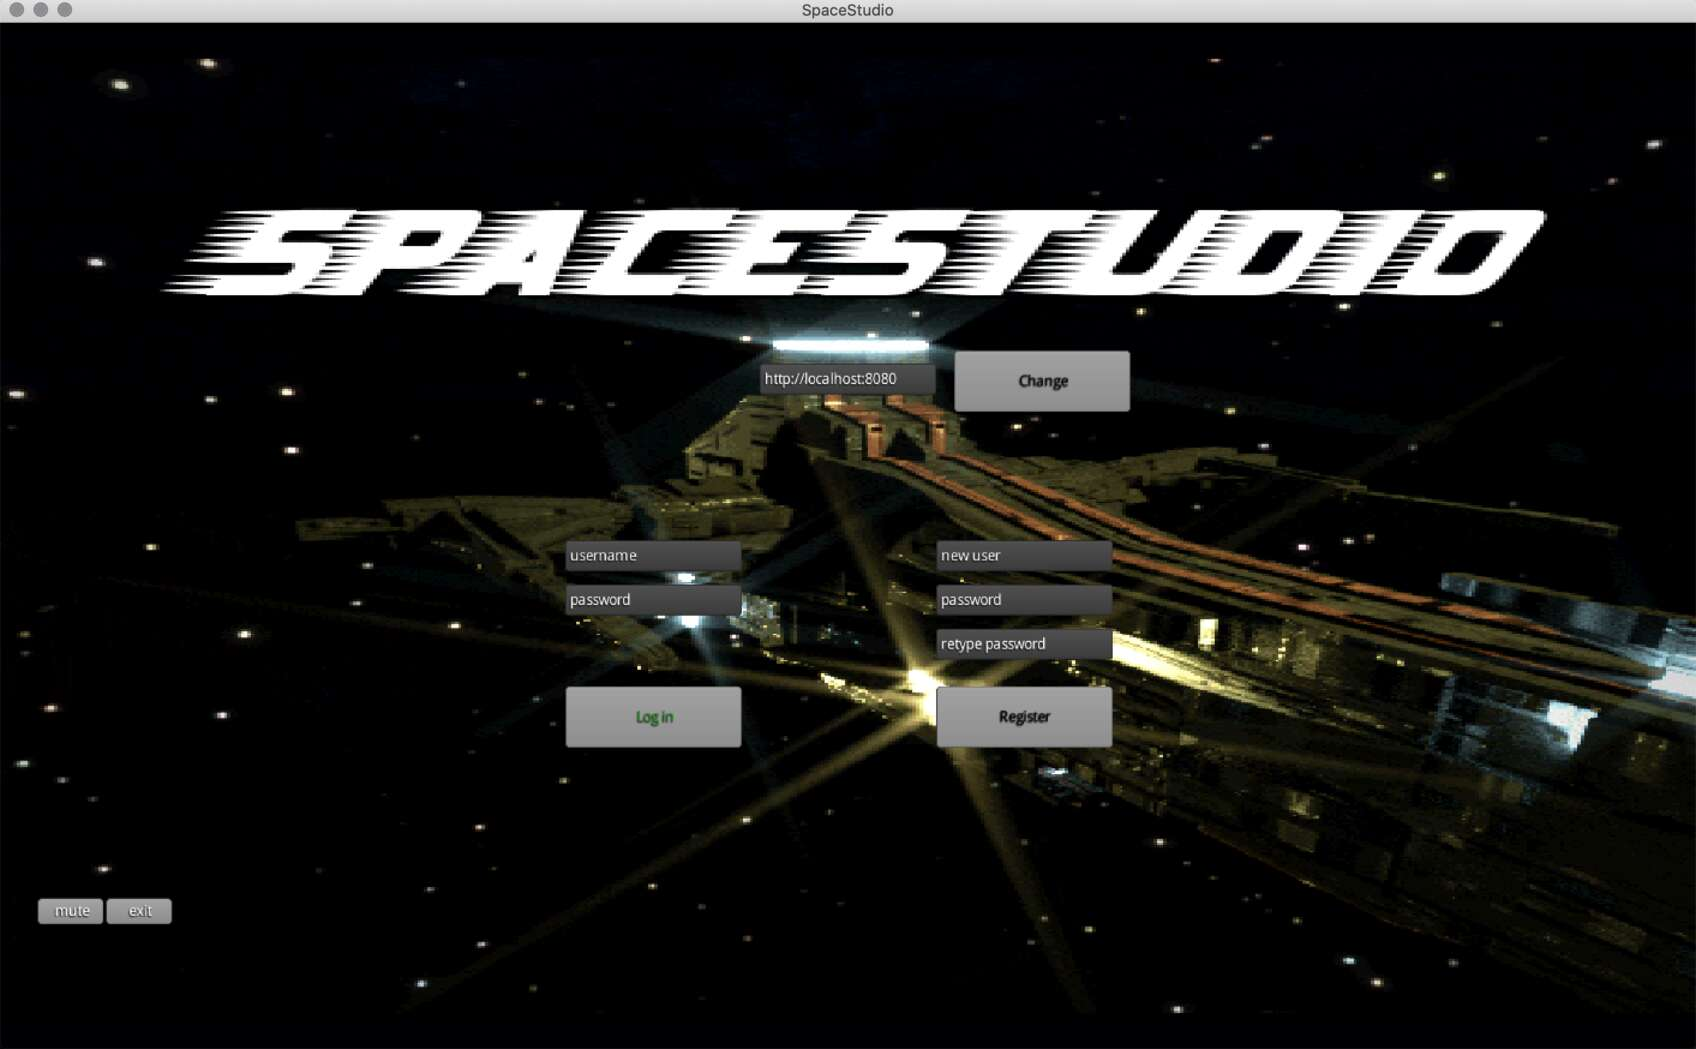
\includegraphics[scale=0.4]{TestProtocolBilder/startScreen.jpg}
\caption{Start Screen}
\end{figure}

\newpage
\subsubsection{Erfolgreiche/Fehlerhafte  Registrierung}
Wenn der Benutzer die Felder korrekt eingegeben hat, erhält er eine grüne Rückmeldung, in der sich die Bestätigungsnachricht des Servers für die Erstellung seiner Instanz befindet.\\
\begin{figure}[h]
\centering
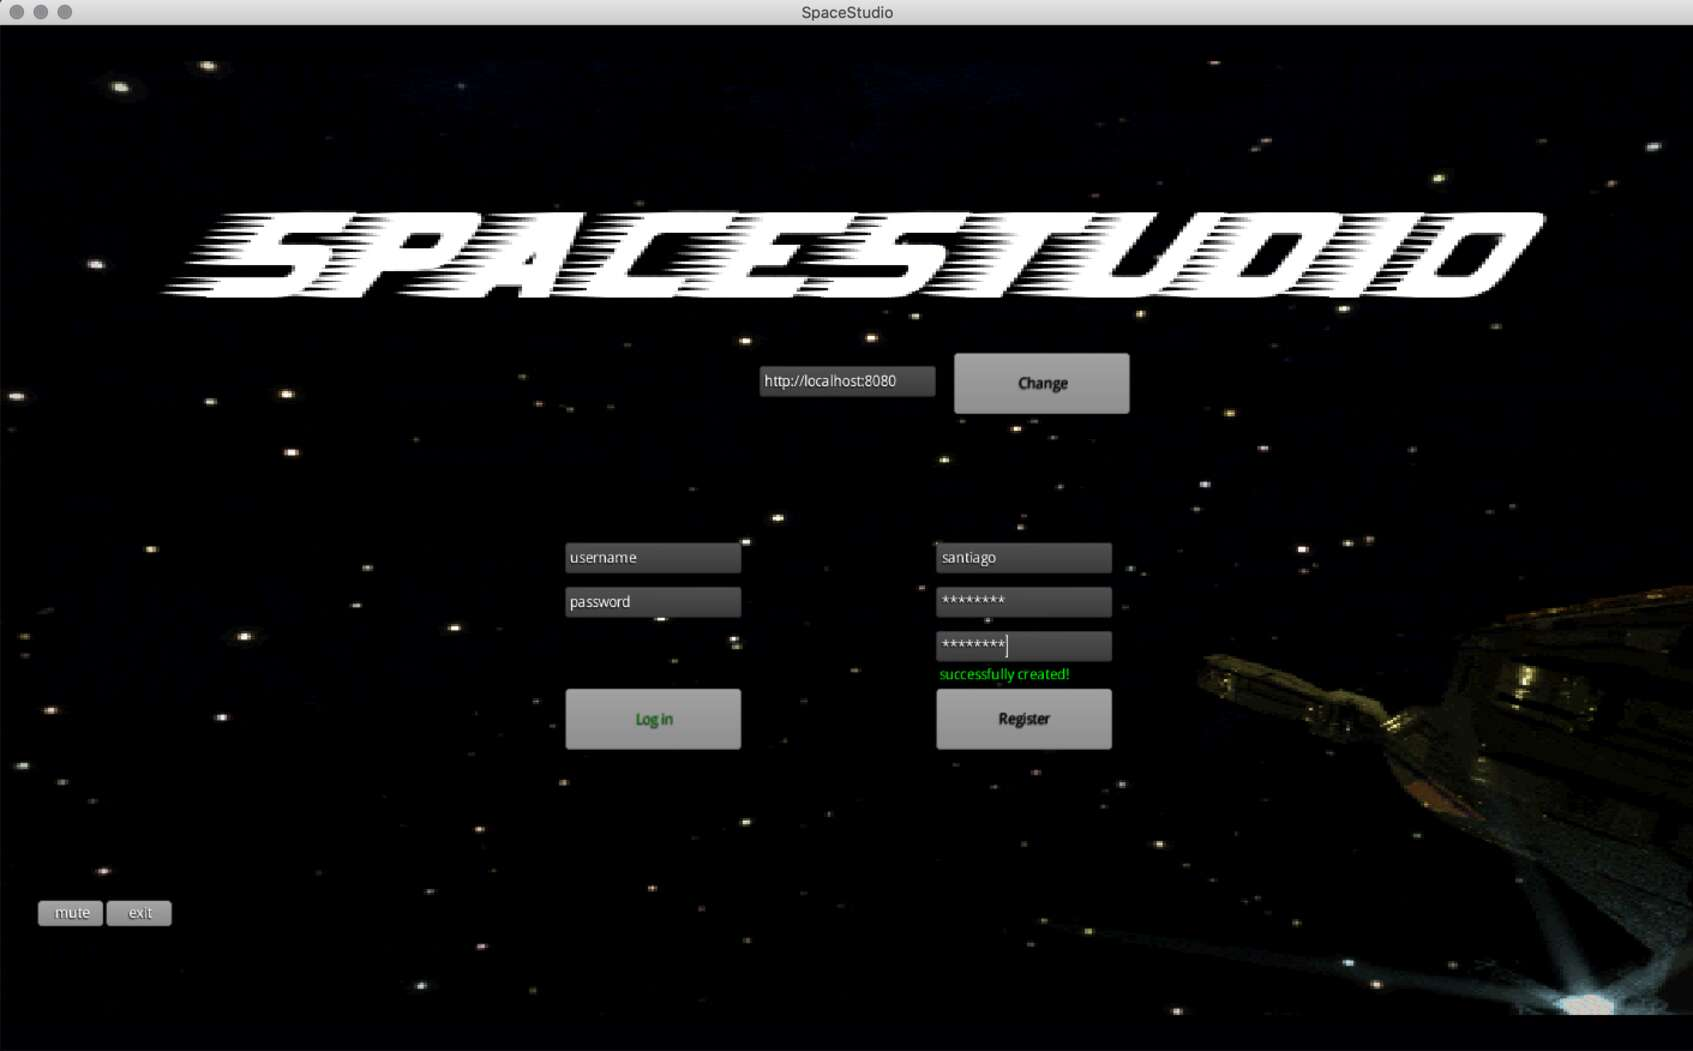
\includegraphics[scale=0.4]{TestProtocolBilder/erfolgAnmelden.jpg}
\caption{Erfolg Anmelden}
\end{figure}

Wenn der Benutzer fehlerhafte, bereits vorhandene oder unvollständige Daten in die Registrierungsfelder schreibt, erhält er eine negative Rückmeldung, in der das Problem dargestellt wird, auf das der Server beim Speichern der Daten gestoßen ist.\\
\begin{figure}[h]
\centering
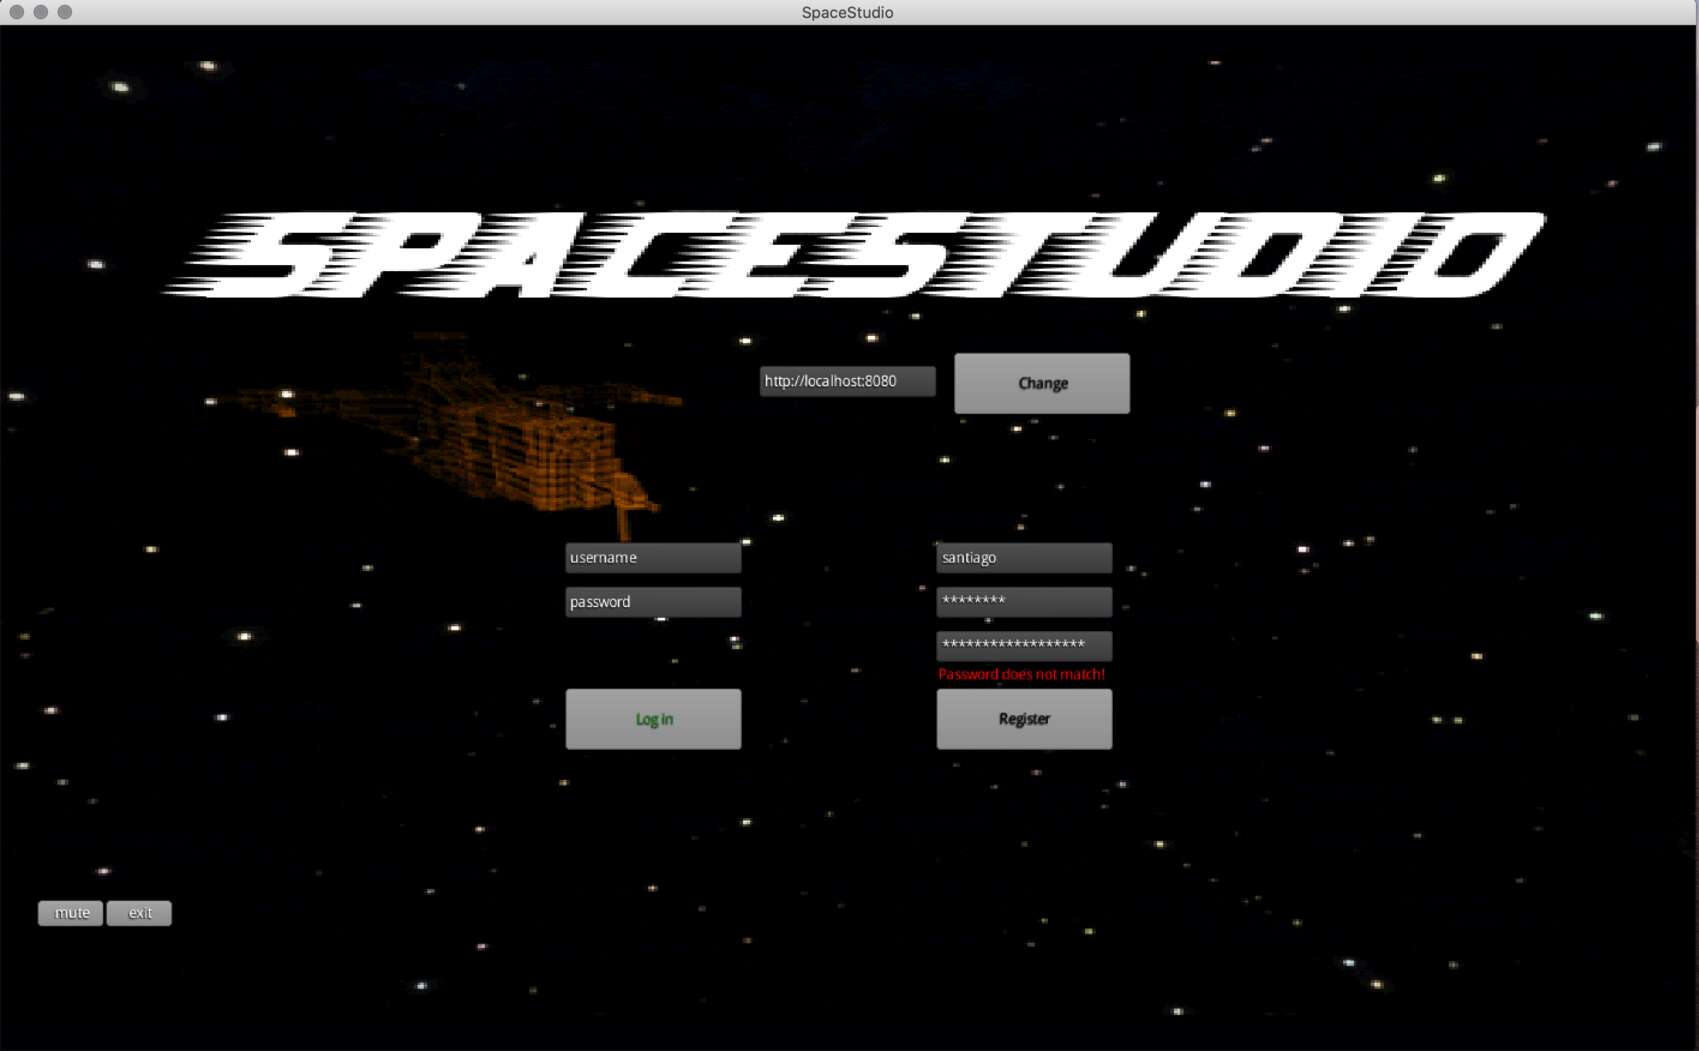
\includegraphics[scale=0.4]{TestProtocolBilder/doesnotMatchPassword.jpg}
\caption{Ungültiger Name oder Passwort}
\end{figure}
\newpage
\subsubsection{Erfolgreiche Registrierung}
Wenn sich der Benutzer mit dem richtigen Namen und Passwort registriert hat, überprüft der Server die Daten und speichert diese in der Datenbank.\\

\begin{figure}[h]
\centering
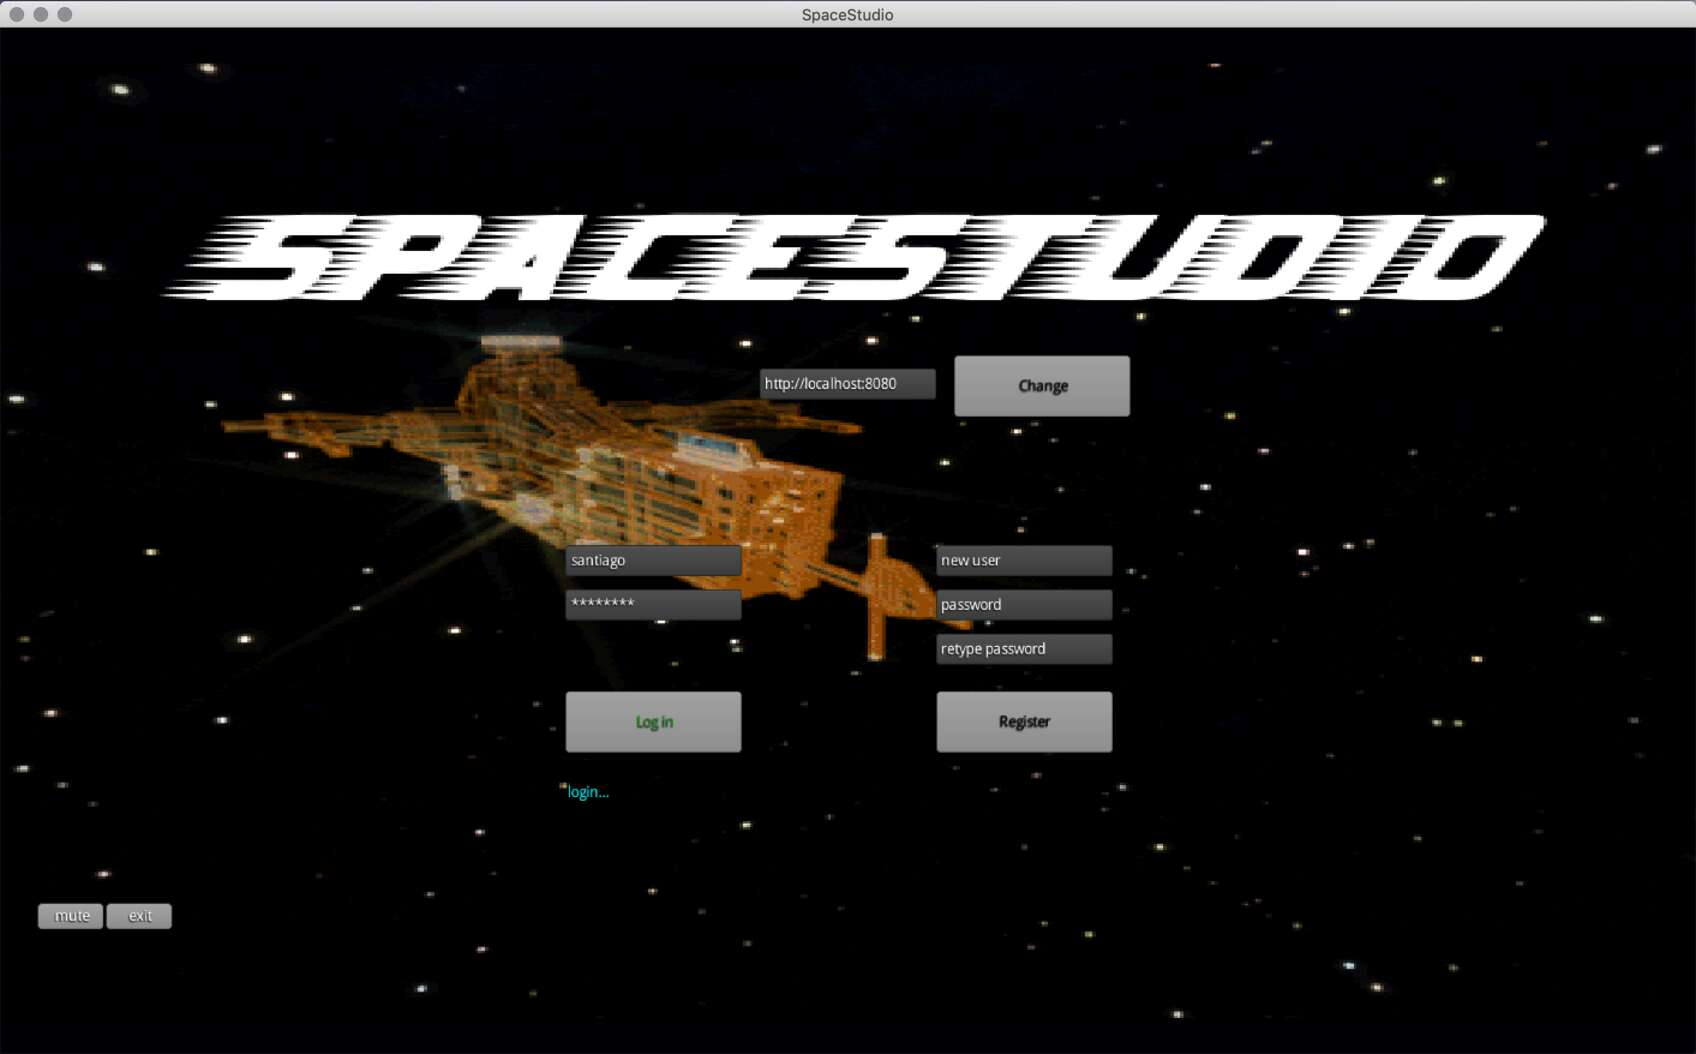
\includegraphics[scale=0.4]{TestProtocolBilder/erfolgLogin.jpg}
\caption{Login Erfolg}
\end{figure}
\newpage
\subsection{Anmeldung}
\subsubsection{Fehlerhafte Anmeldung}
Wenn sich der Benutzer mit falschen Daten angemeldet hat, kann der Server den Benutzer nicht validieren, sodass er nicht zum nächsten Bildschirm weitergeleitet werden kann.
\begin{figure}[h]
\centering
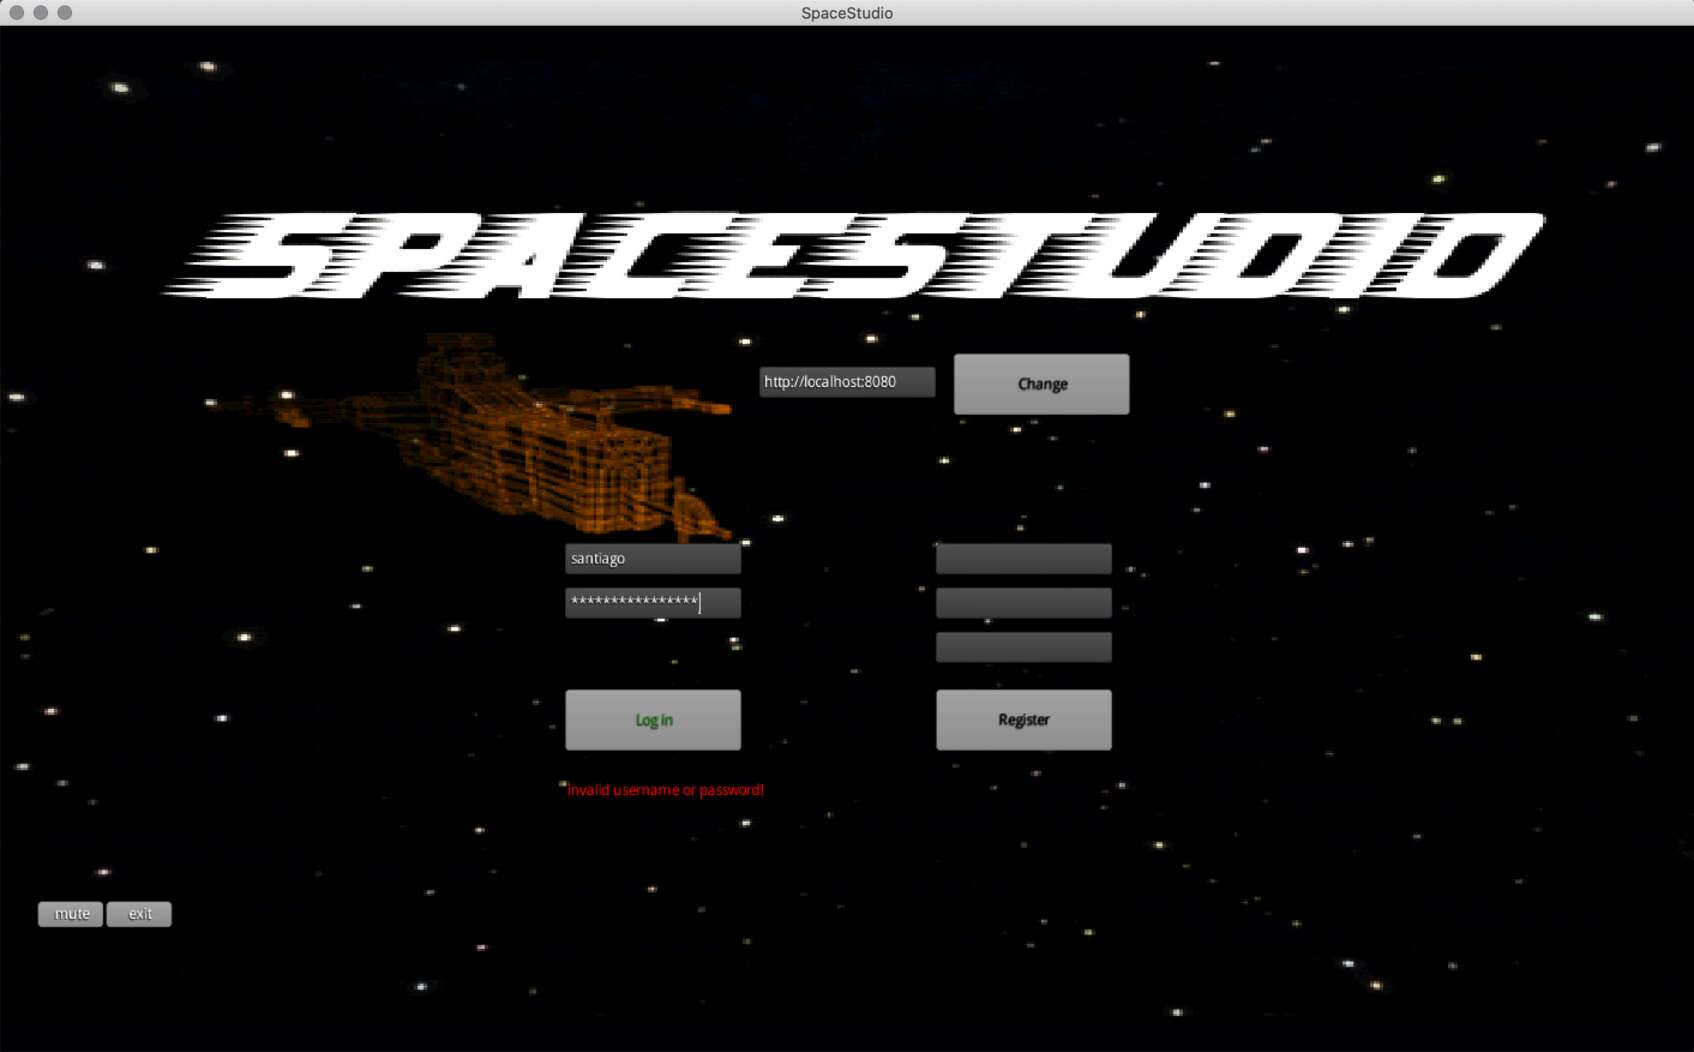
\includegraphics[scale=0.4]{TestProtocolBilder/invalidCredentials.jpg}
\caption{Ungültige Zugangsdaten}
\end{figure}
\newpage
Wenn sich der Benutzer mit den richtigen Anmeldeinformationen anmeldet hat, wird der Benutzer zum Menübildschirm weitergeleitet.\\

\section{Menü Screen}
Auf dem Menübildschirm sind die Optionen:
\begin{itemize}
\item Continue: Falls ein Spielstand für den Benutzer in der Datenbank gespeichert wurde, wird auch die Option Continue angezeigt. Mit der kann der Benutzer in seinen vorhandenen Spielstand wechseln.
\item New Game: Mit dieser Option kann der Benutzer ein neues Spiel starten
\item About: In dieser Option können Informationen zu den Entwicklern gefunden werden.
\item Exit: Mit dieser Option kann der Benutzer das Spiel beenden.
\end{itemize}
\begin{figure}[htp]
\centering
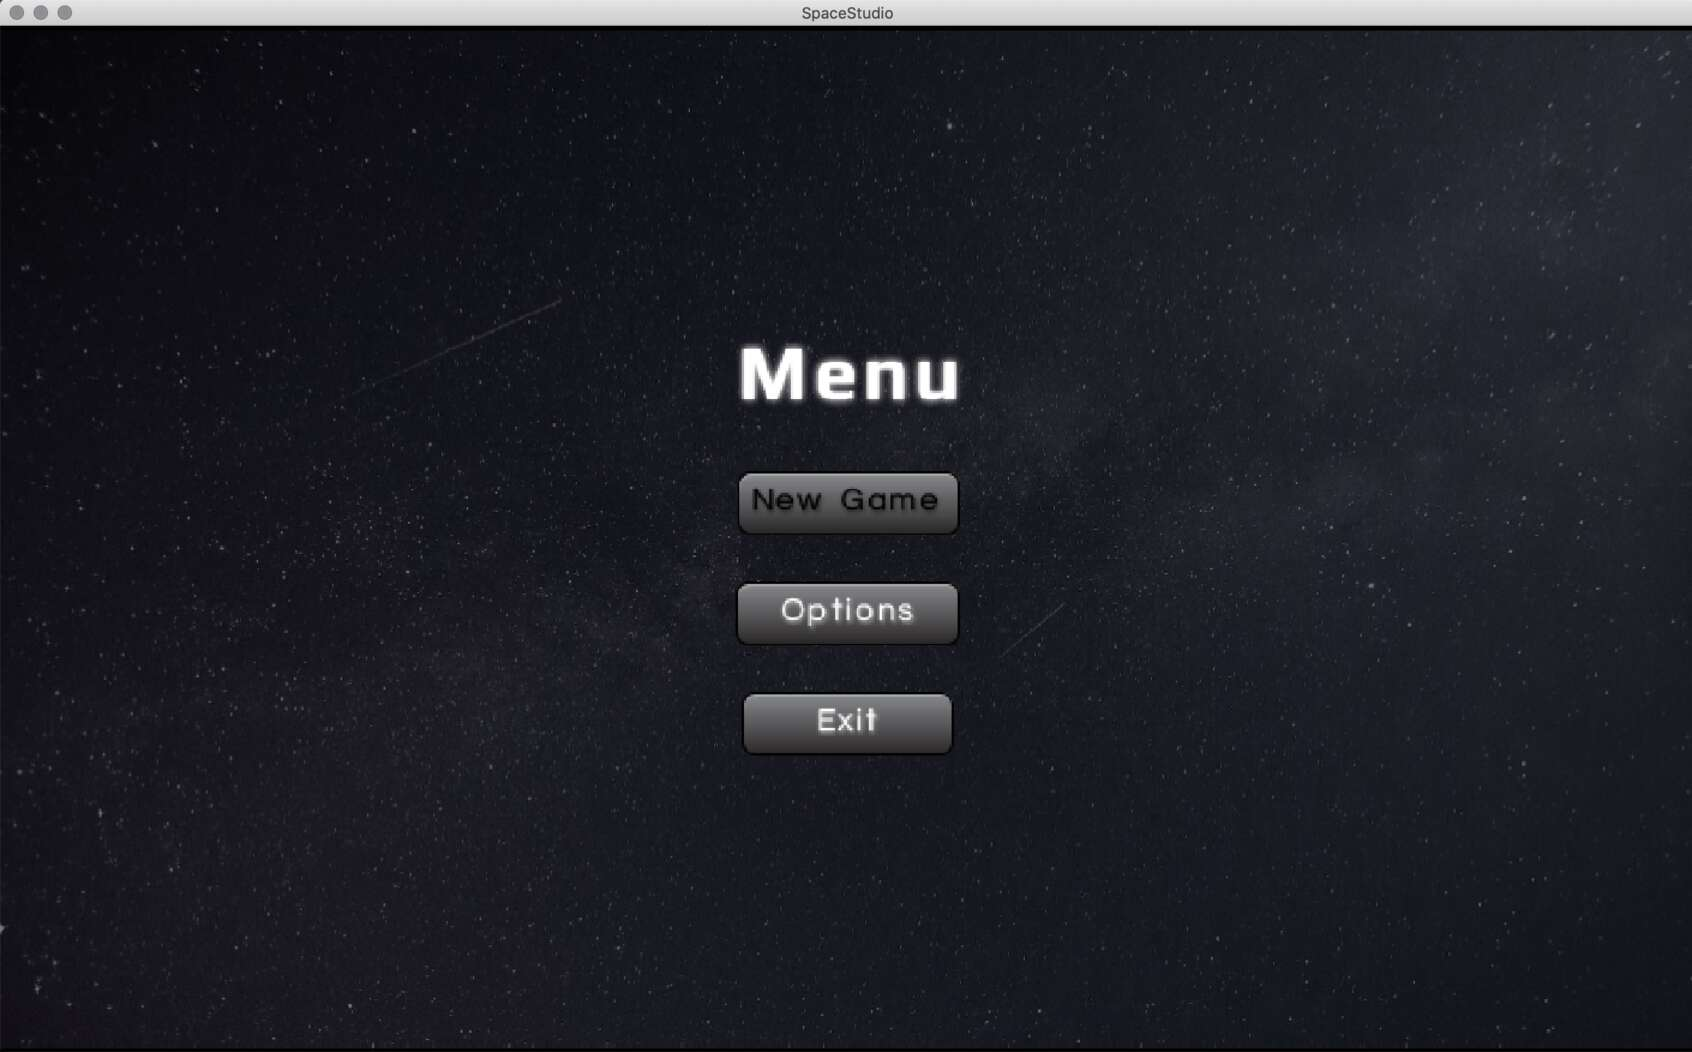
\includegraphics[scale=0.4]{TestProtocolBilder/menuScreen.jpg}
\caption{Menu Spiel}
\end{figure}
\newpage
\section{Spieloptionen}
Im zweiten Menübildschirm können Sie die Optionen sehen, die der Benutzer spielen muss.
\begin{itemize}
\item Single Player: Mit dieser Option kann der Benutzer als Einzelspieler im Universum spielen.
\item Multiplayer: Diese Option ermöglicht es dem Benutzer, mit einem anderen Spieler im Universum zu spielen und gegeneinander zu kämpfen.
\item Back to Menu: Diese Option ermöglicht es Ihnen, zum vorherigen Bildschirm zurückzukehren.
\end{itemize}
\begin{figure}[h]
\centering
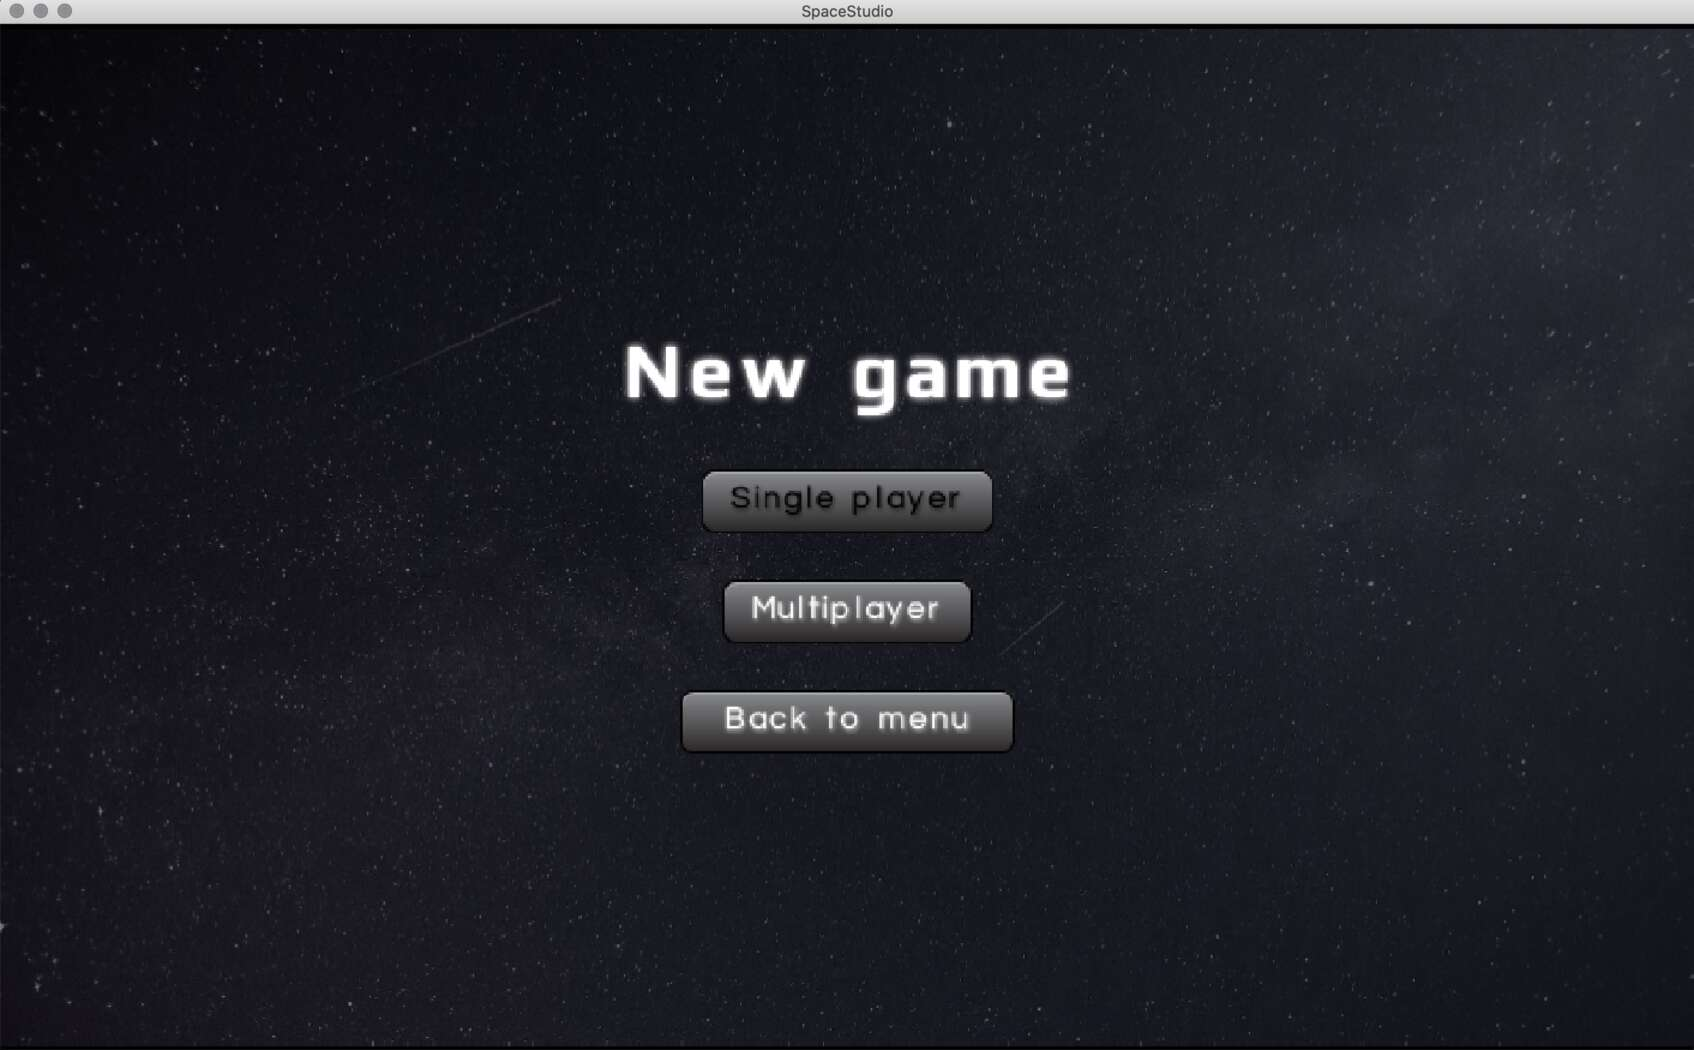
\includegraphics[scale=0.4]{TestProtocolBilder/menuScreenTwo.jpg}
\caption{Spieloptionen}
\end{figure}
\newpage
\section{Testfall Single Player}
Auf diesem Bildschirm wurde jede Schaltfläche getestet, beginnend mit der Taste Single Player.\\
\begin{figure}[h]
\centering
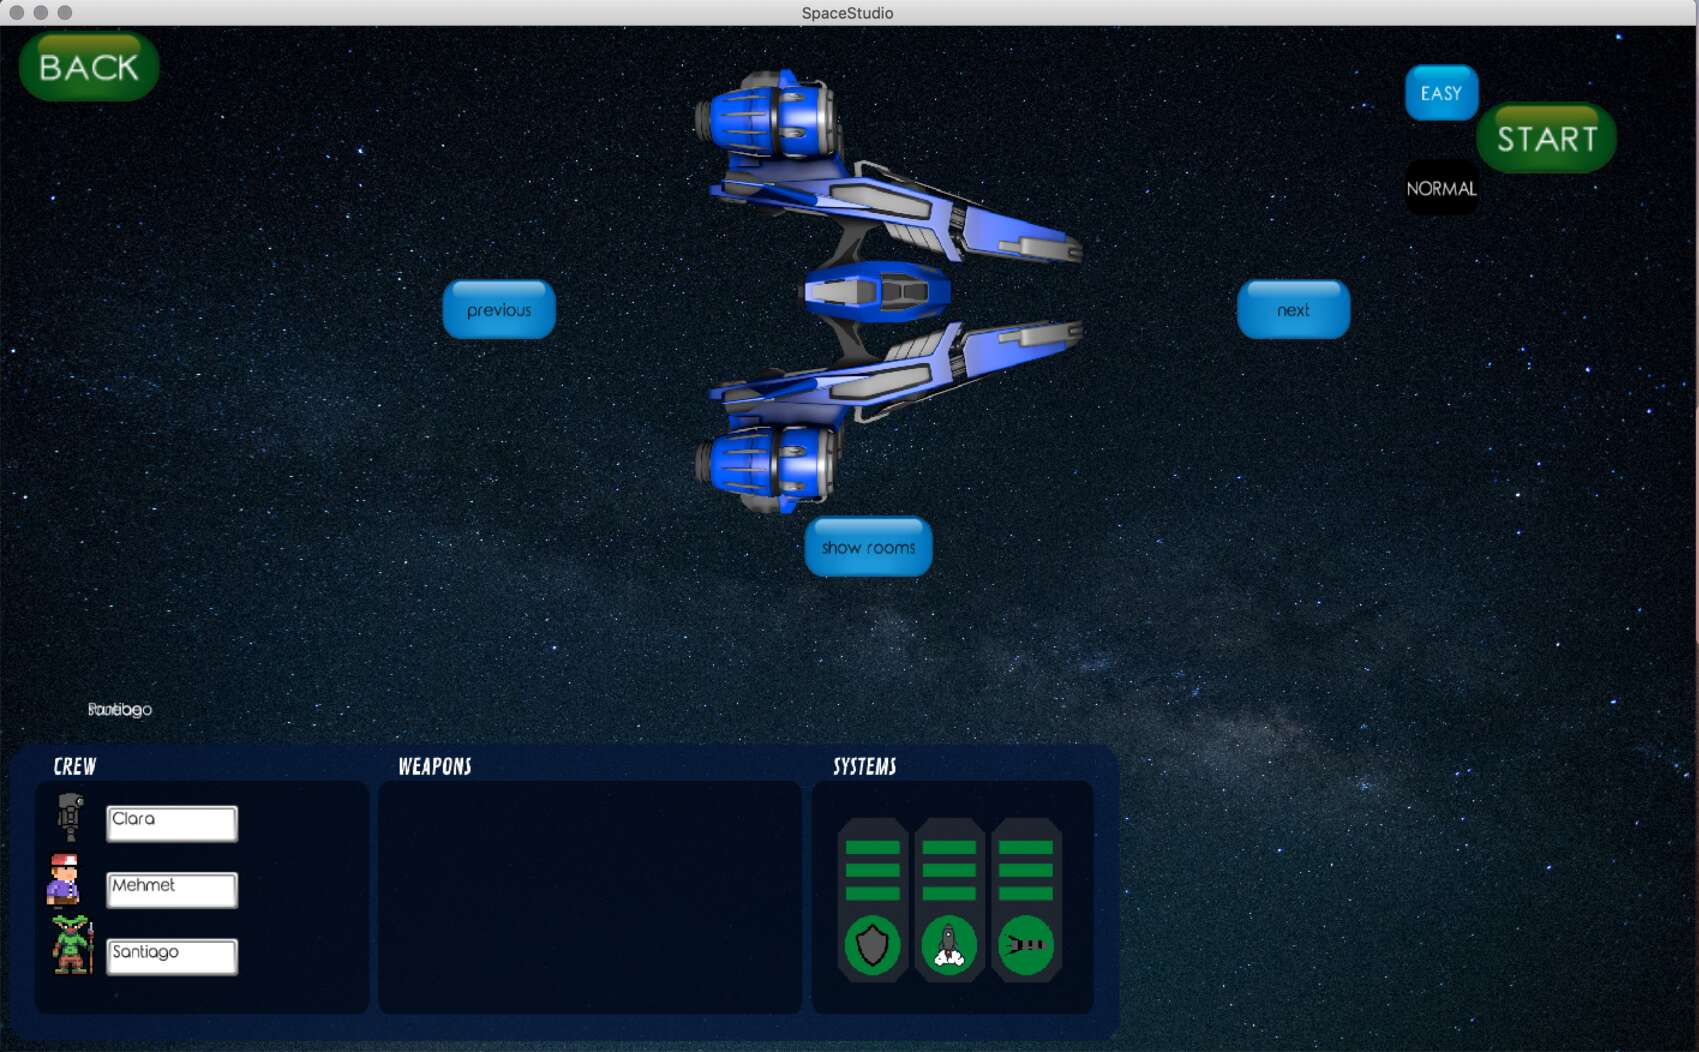
\includegraphics[scale=0.4]{TestProtocolBilder/selecShipScreen.jpg}
\caption{Select Ship screen}
\end{figure}
\newpage
\subsection{Sektionen anzeigen Test}

Mit dem Button "show rooms" wurde getestet, ob die Sektionen des Raumschiffes sichtbar sind. Wenn Sie erneut drücken, verschwinden die Abschnitte\\
\begin{figure}
\centering
\includegraphics[scale=0.4]{TestProtocolBilder/shipRooms.jpg}
\caption{Sektionen des Raumschiffs}
\end{figure}

\newpage

\subsection{Andere Raumschiffe}
Mit der nächsten Schaltfläche kann der Benutzer die möglichen Schiffe für das Spiel sehen.
\begin{figure}
\centering
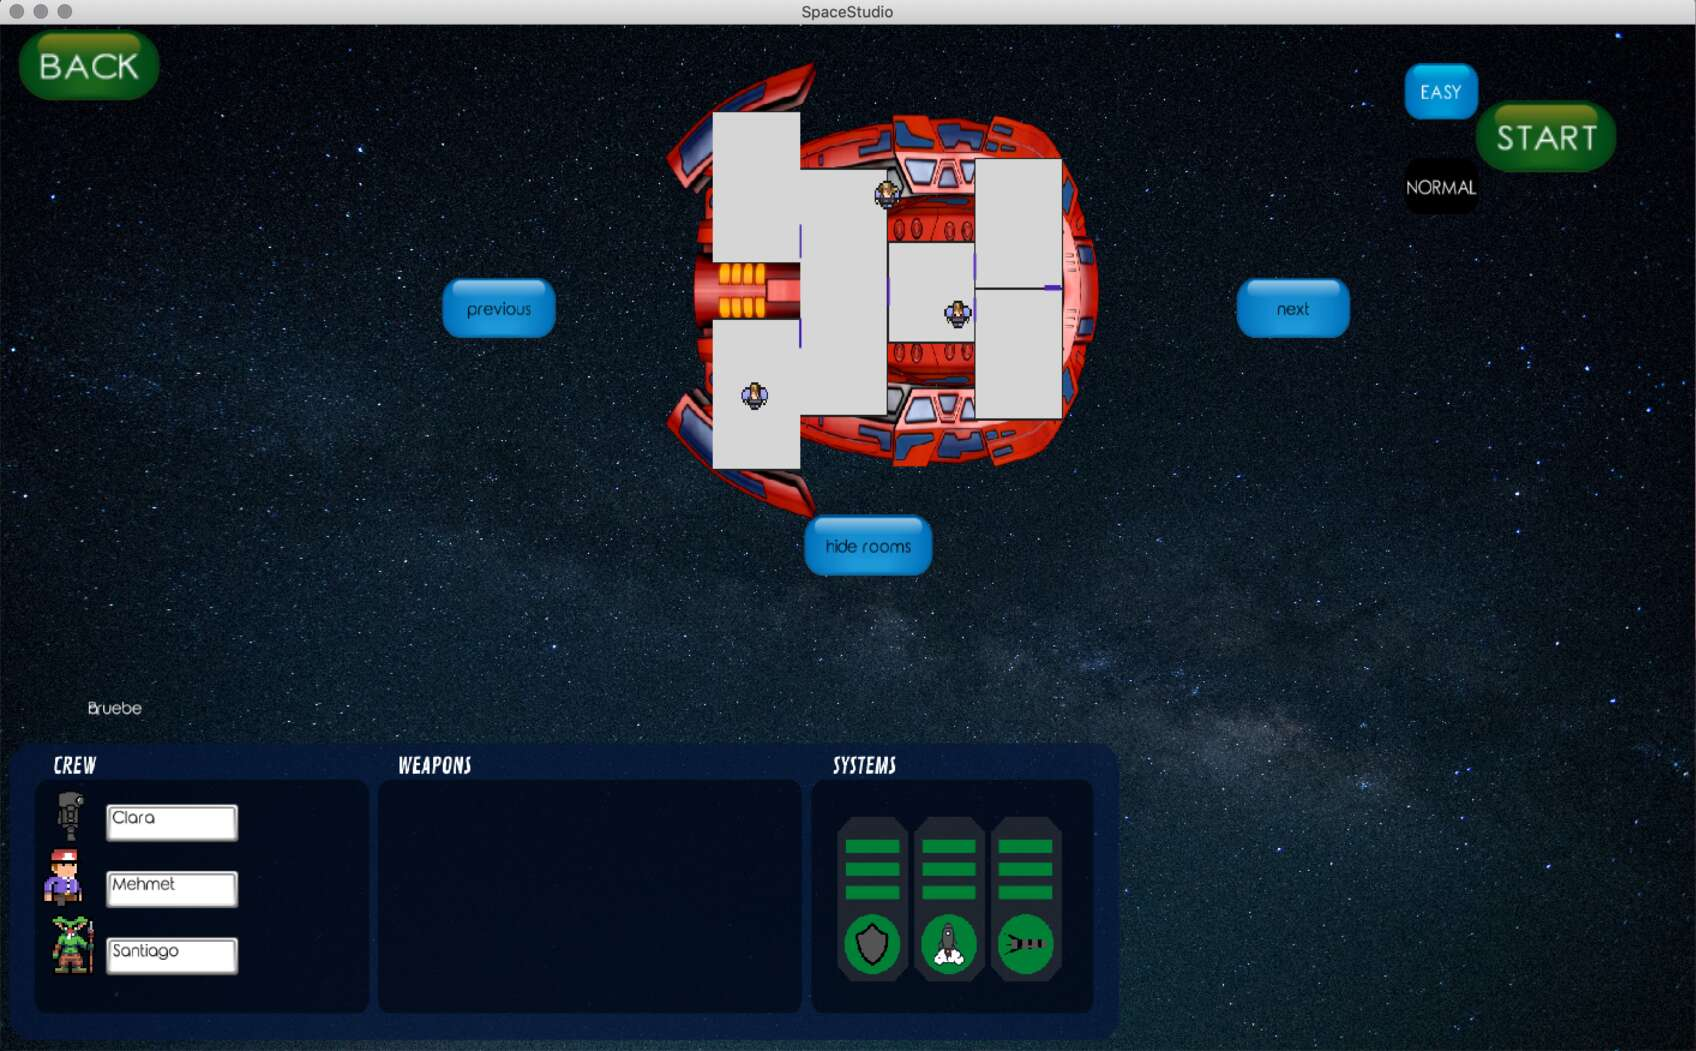
\includegraphics[scale=0.4]{TestProtocolBilder/next.jpg}
\caption{Andere mögliche Raumschiffe}
\end{figure}

\newpage
\subsection{Universum Schwierigkeit}

Diese Testschaltfläche ermöglicht die Schaffung eines größeren Universums, in dem es mehr Planeten mit unterschiedlichen Eigenschaften gibt.\\
\begin{figure}
\centering
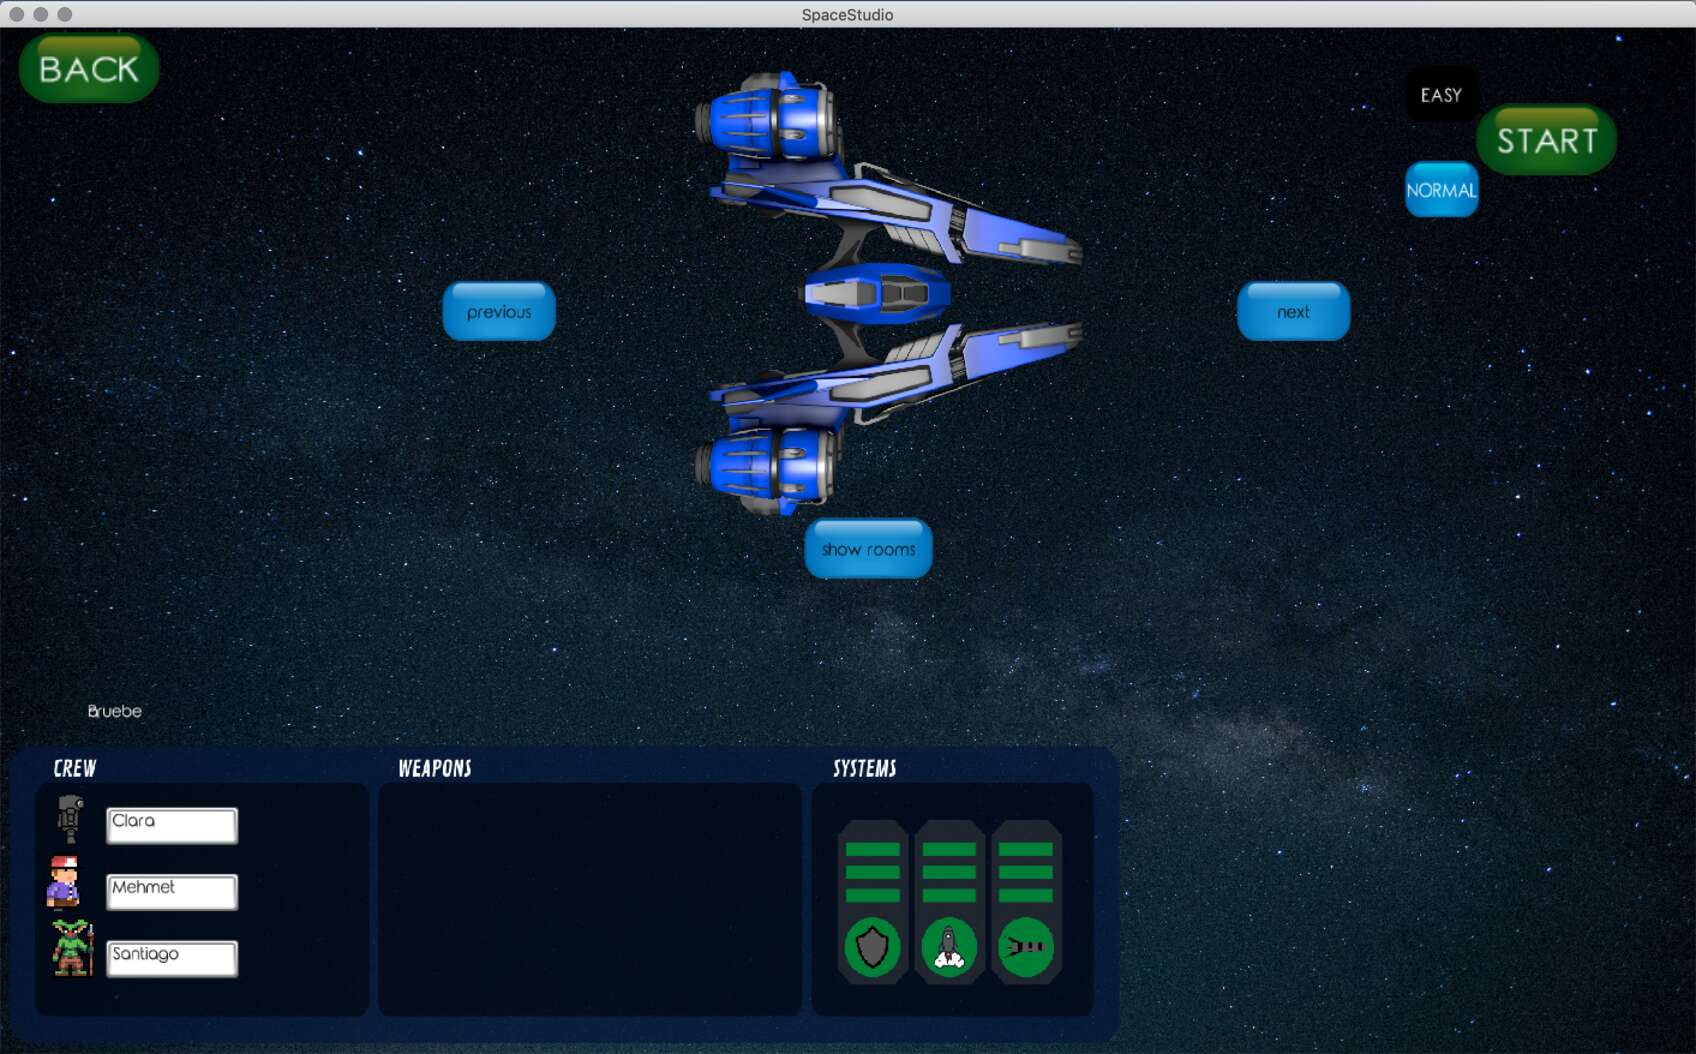
\includegraphics[scale=0.4]{TestProtocolBilder/universeButon.jpg}
\caption{Leichte und normale Schwierigkeit}
\end{figure}

\newpage
Das Universum mit einer komplexeren Schwierigkeit wird korrekt erstellt.\\

\begin{figure}[t]
\centering
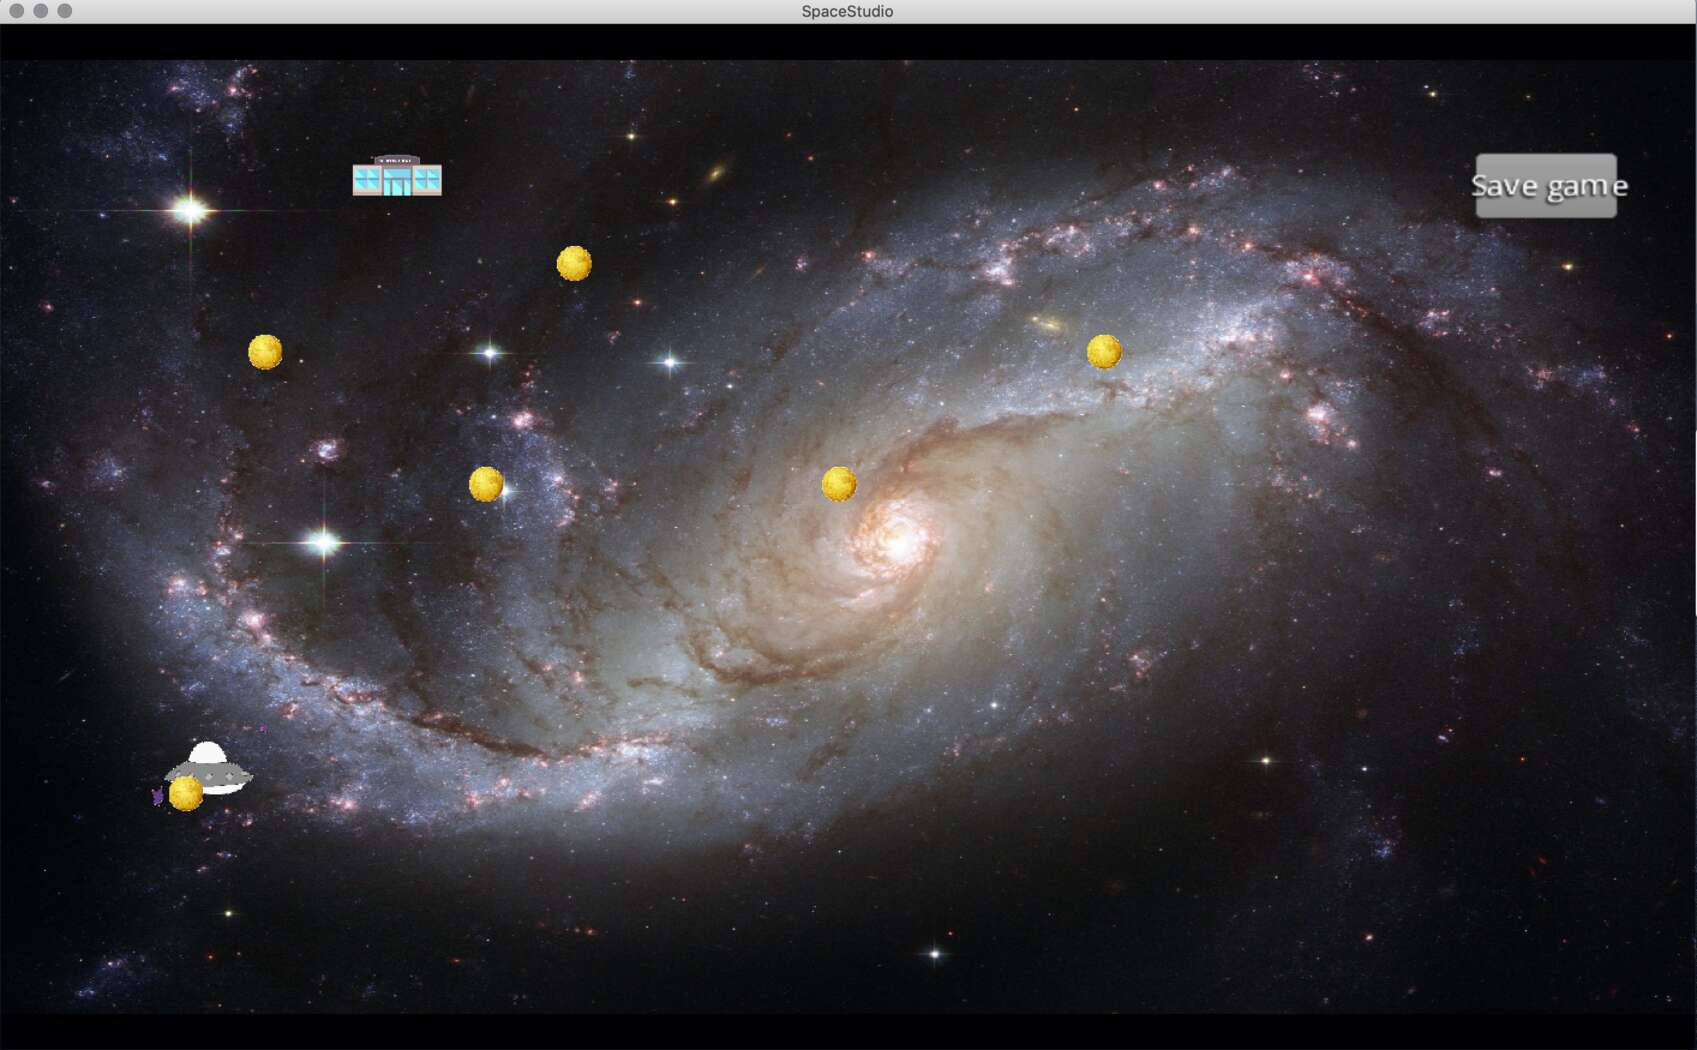
\includegraphics[scale=0.4]{TestProtocolBilder/universeHard.jpg}
\caption{Universum normal Schwierigkeit}
\end{figure}

Die Schaltfläche, die das Beenden des Universums erleichtert, wurde ebenfalls getestet.\\

\begin{figure}[t]
\centering
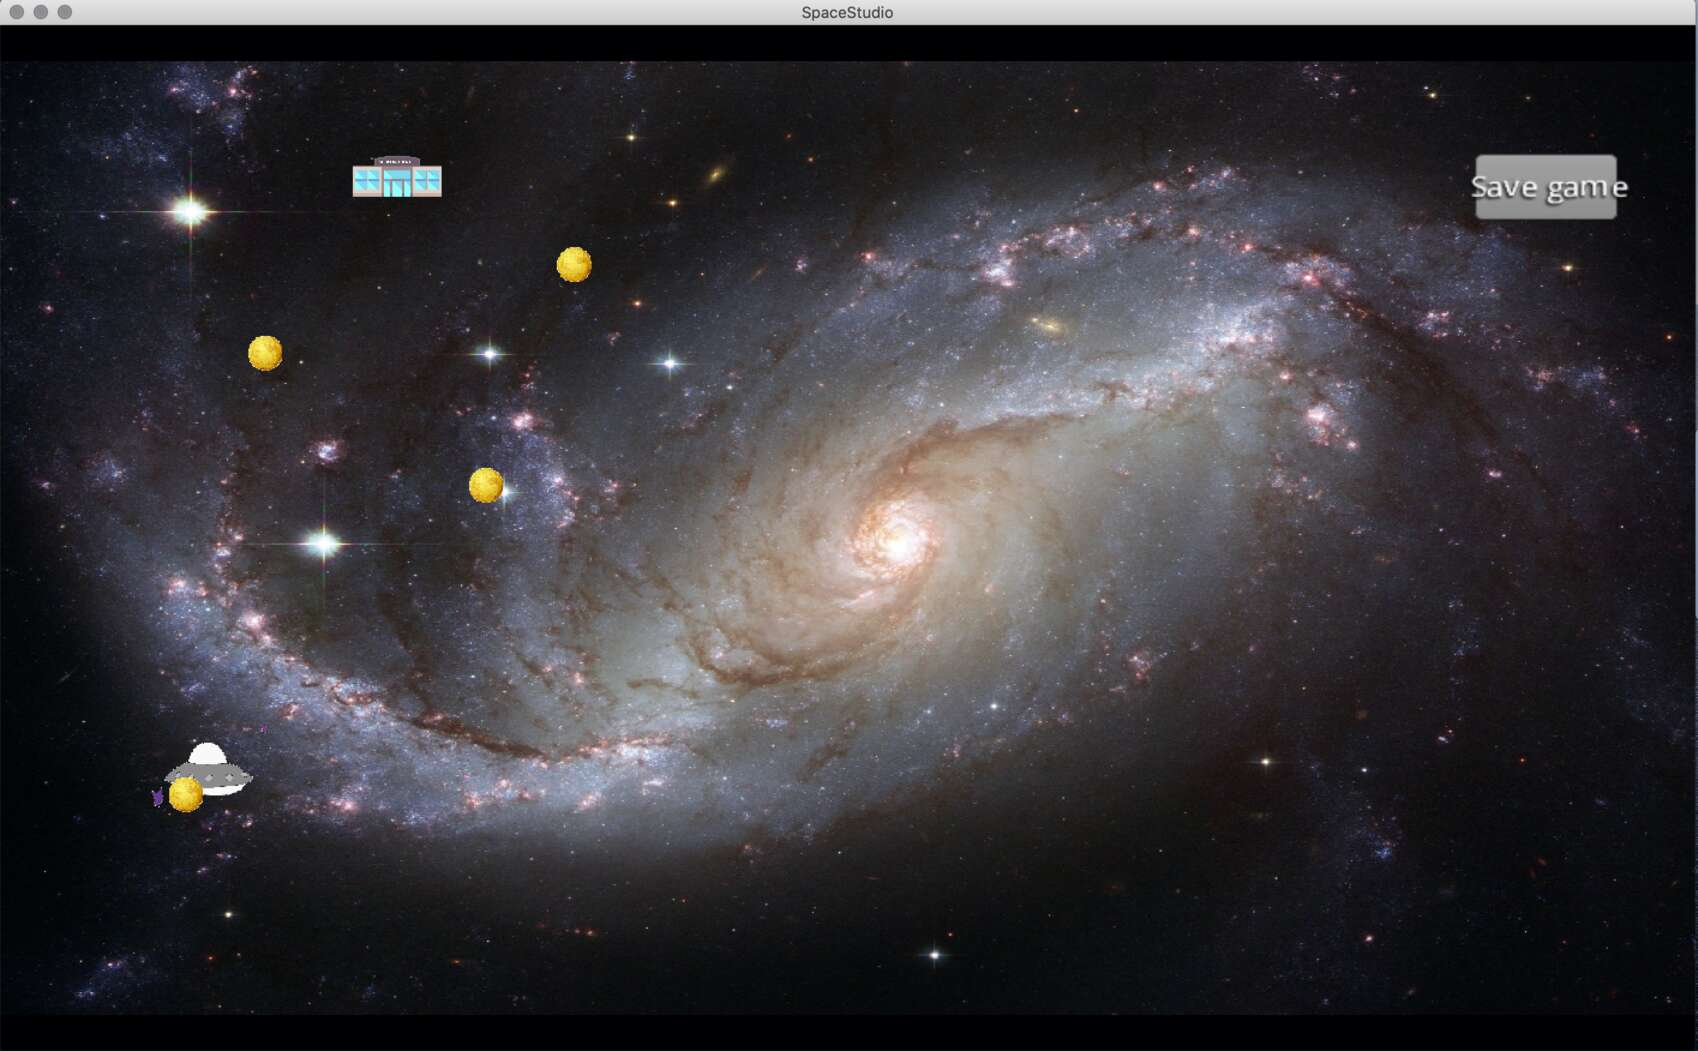
\includegraphics[scale=0.4]{TestProtocolBilder/universeEase.jpg}
\caption{Universum im leichten Schwierigkeitsmodus}
\end{figure}

\newpage
\subsection{Karte}

Hier wurde jeder Planet und jede Station getestet, die Schaltflächen sind der Zugang zum Ereignis-Bildschirm.\\
\begin{figure}
\centering
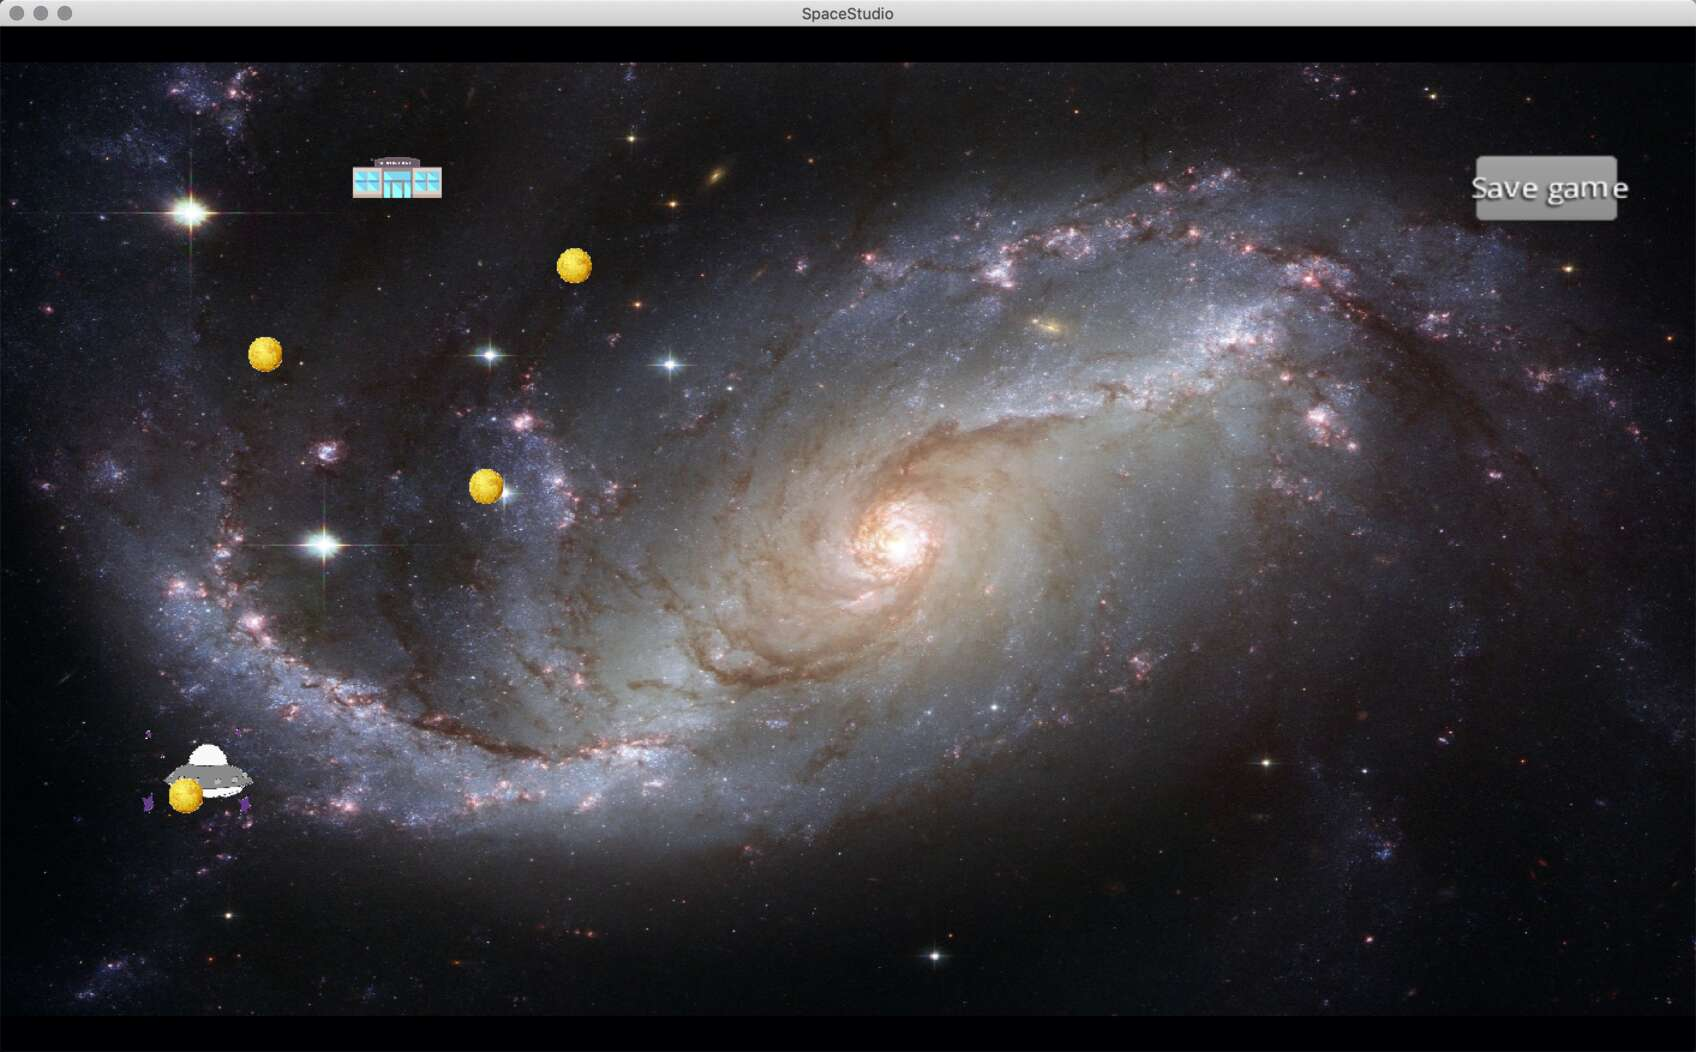
\includegraphics[scale=0.4]{TestProtocolBilder/map.jpg}
\caption{Game Map}
\end{figure}
\newpage
\section{Ereignisse}
Nach dem Drücken eines Planeten wird ein Popup-Menü angezeigt und die Springfunktion getestet. Nach Auswahl der Springfunktion sieht der Benutzer auf dem Bildschirm eine Fahrzeit von 4 Sekunden.
\begin{figure}[htp]
\centering
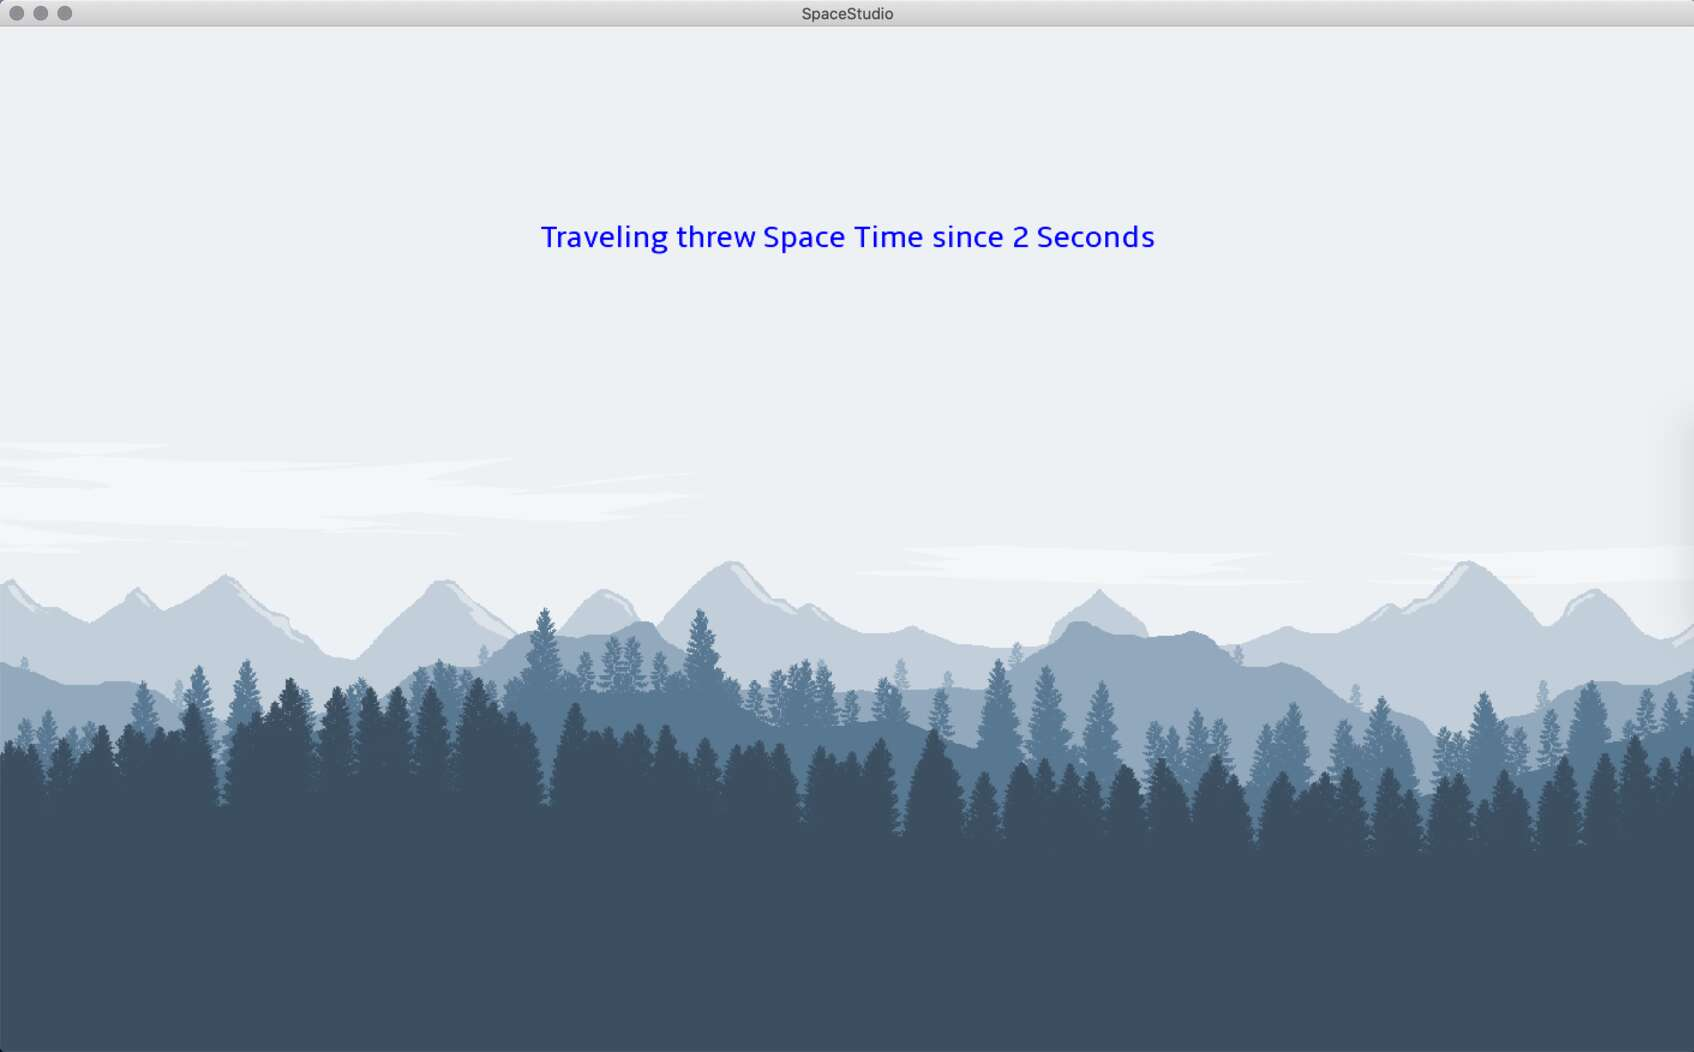
\includegraphics[scale=0.4]{TestProtocolBilder/traveling.jpg}
\caption{Reise Screen}
\end{figure}
Der Button flee, dann man kann wieder auf die Map Screen springen.
\newpage
\subsection{Fliehen}
\begin{figure}[htp]
\centering
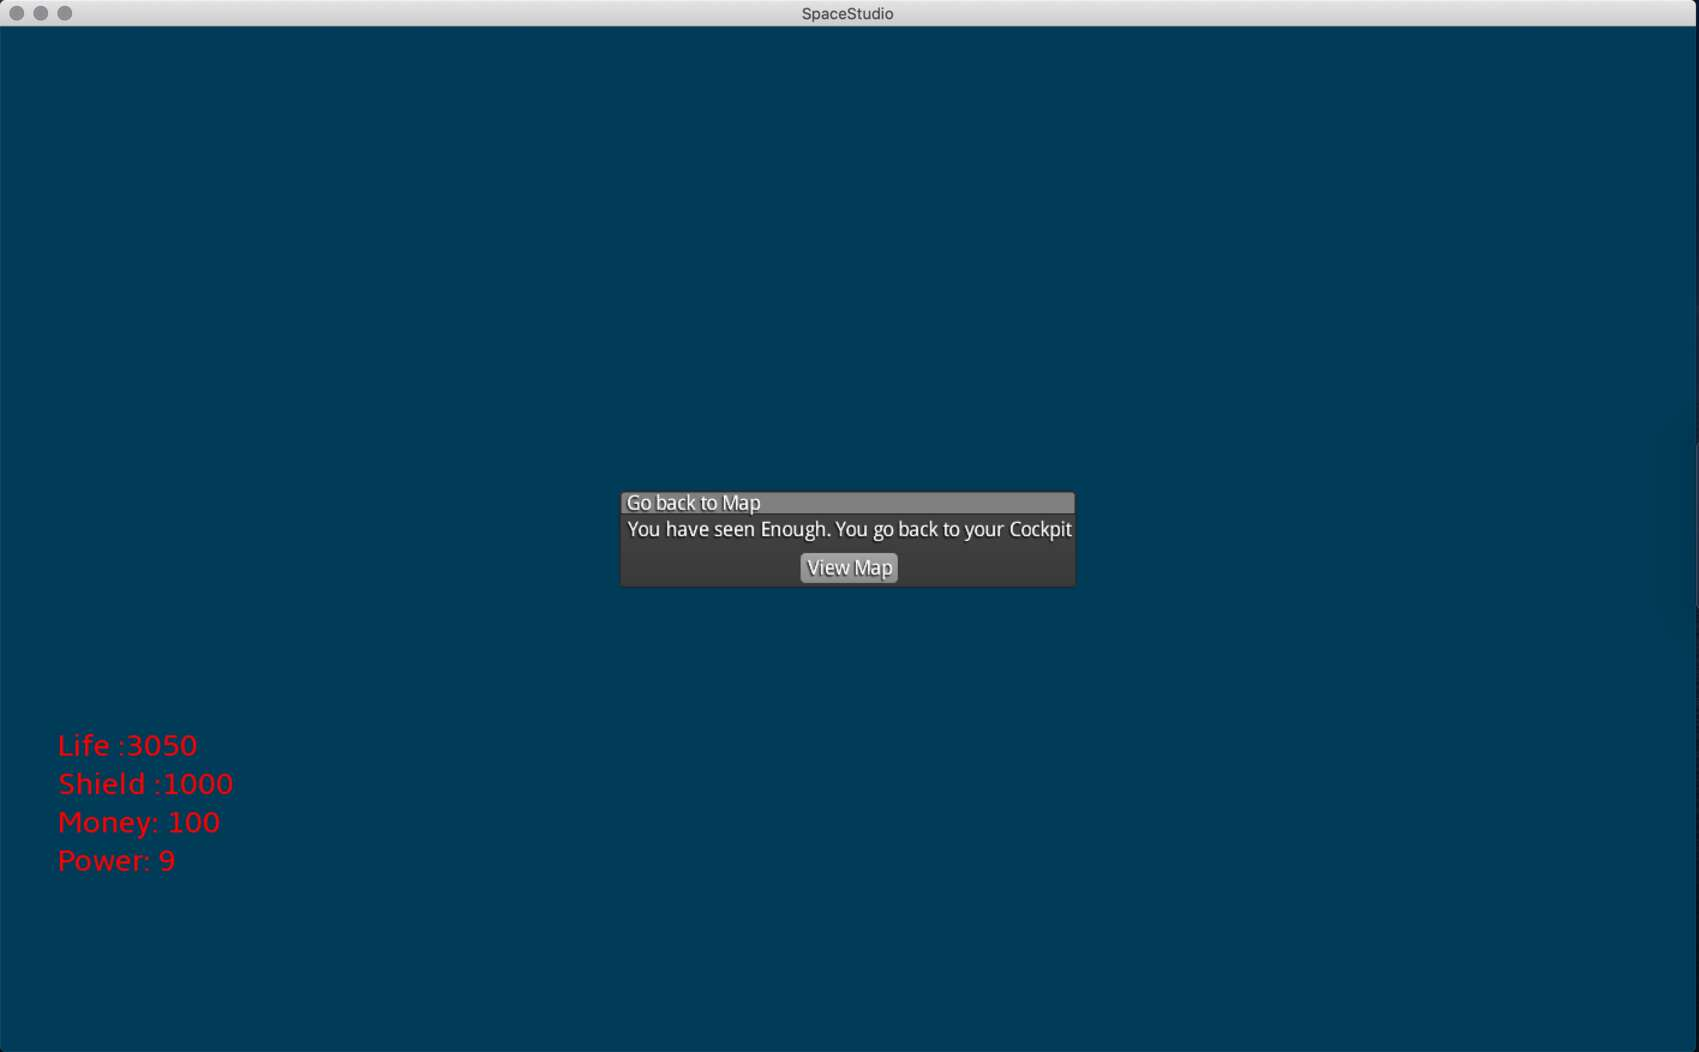
\includegraphics[scale=0.4]{TestProtocolBilder/flee.jpg}
\caption{Fliehen Screen Button}
\end{figure}
\newpage
Es wurde getestet, dass nach dem Reisebildschirm der erste Teil der Ereignisse angezeigt wird.\\
\begin{figure}[htp]
\centering
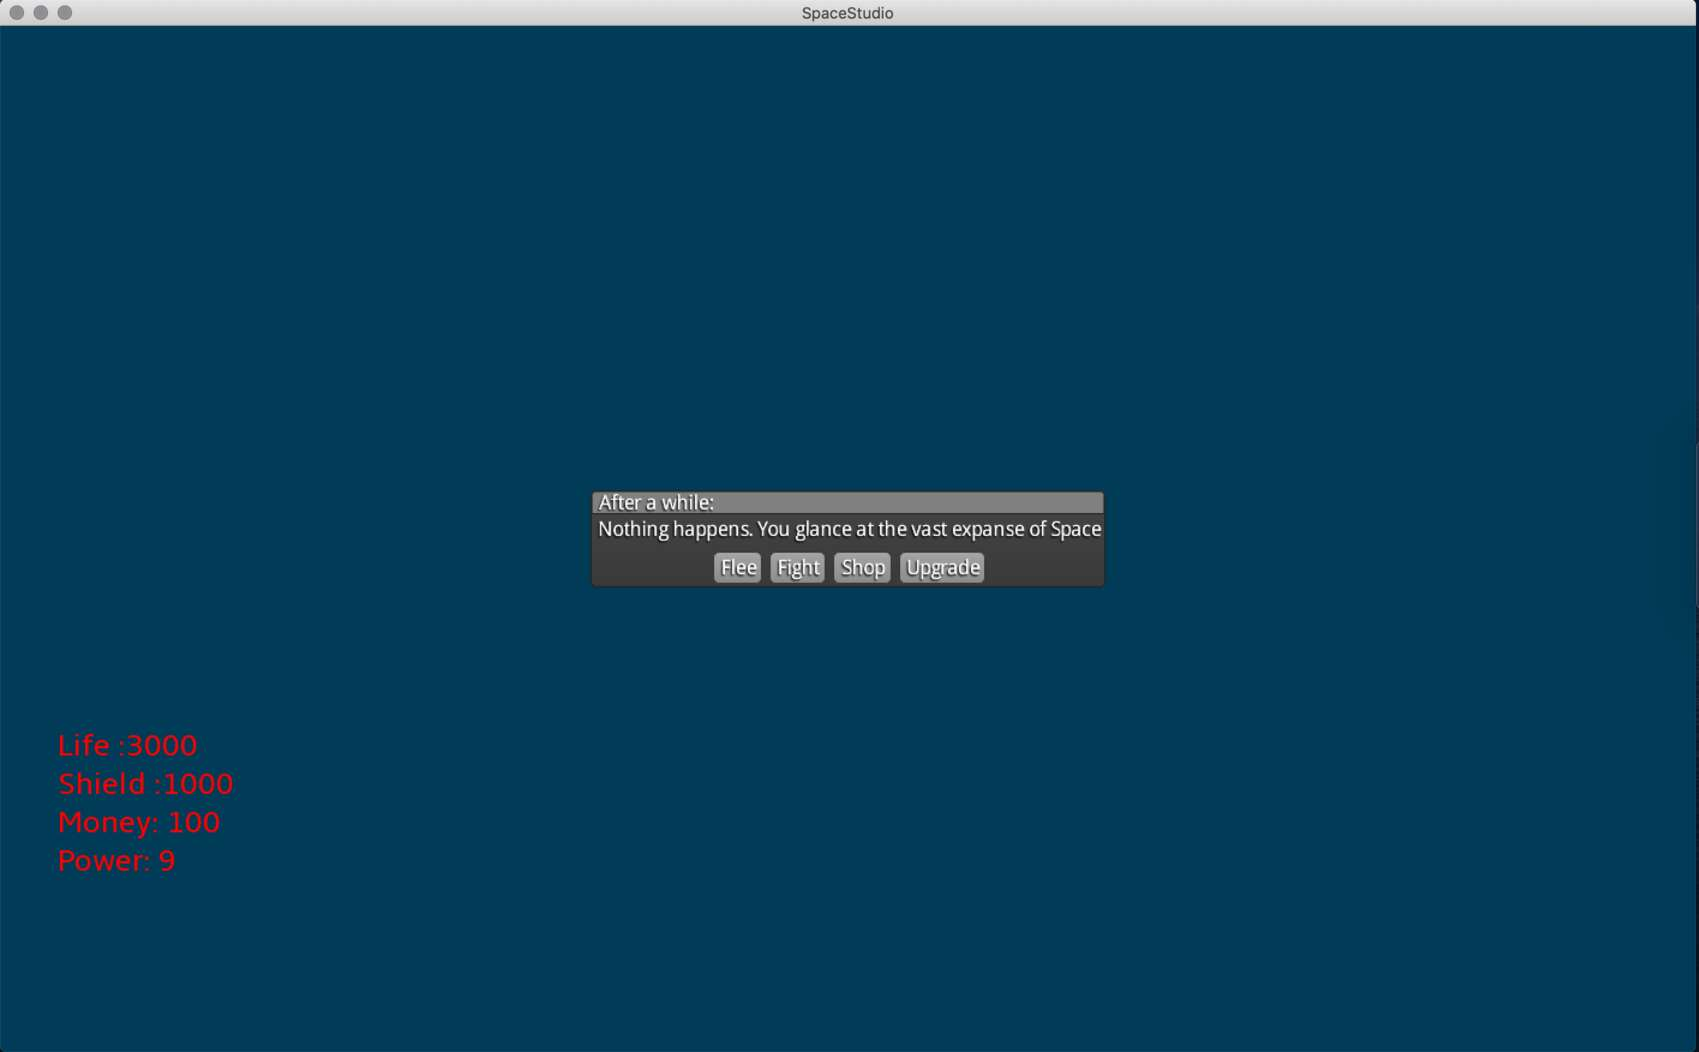
\includegraphics[scale=0.4]{TestProtocolBilder/InitialGeeinisse.jpg}
\caption{Erste Ereignisse}
\end{figure}
Dieser Bildschirm war für die Einführung des Benutzers in die Ereignisse gedacht.
\newpage
Andere Arten von Ereignissen wurden getestet, insgesamt gibt es fünf verschiedene Arten von Ereignissen pro Universum.
\begin{figure}[htp]
\centering
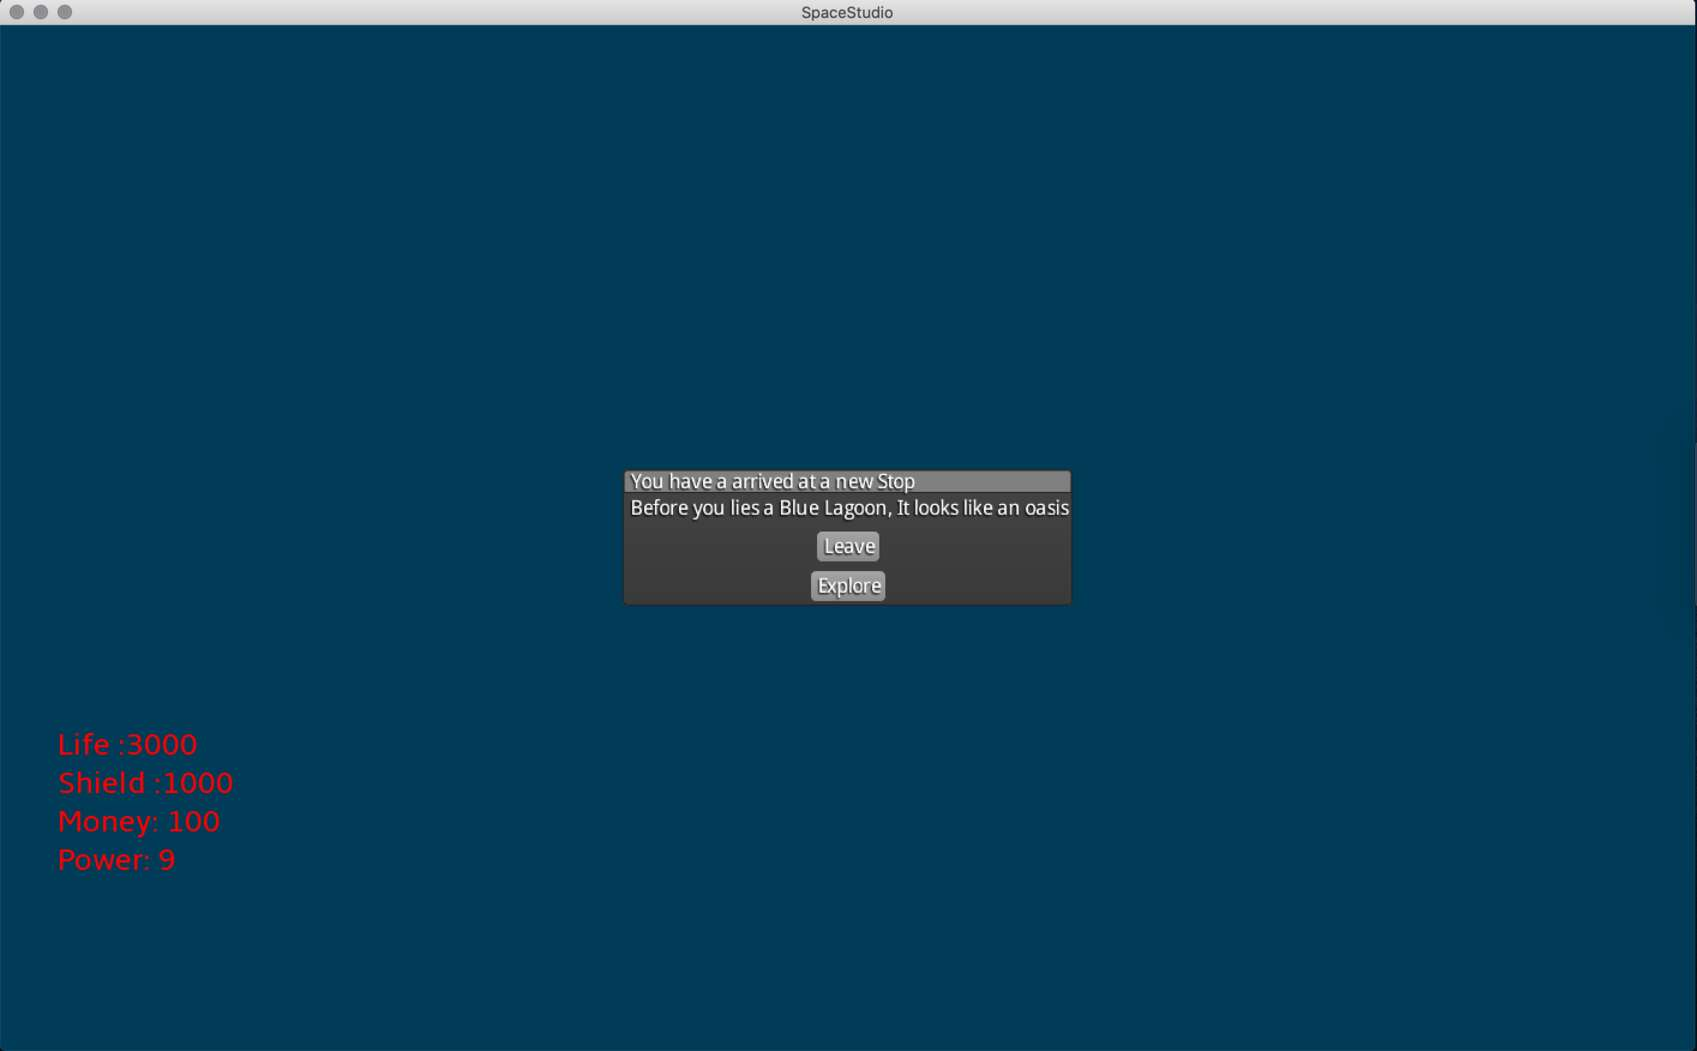
\includegraphics[scale=0.4]{TestProtocolBilder/otherEreignisse.jpg}
\caption{Anderer Typ von Ereignissen}
\end{figure}
Sobald Sie den Einkaufsteil des Spiels betreten, können Sie die in diesem Teil verfügbaren Dinge kaufen.
\begin{figure}[htp]
\centering
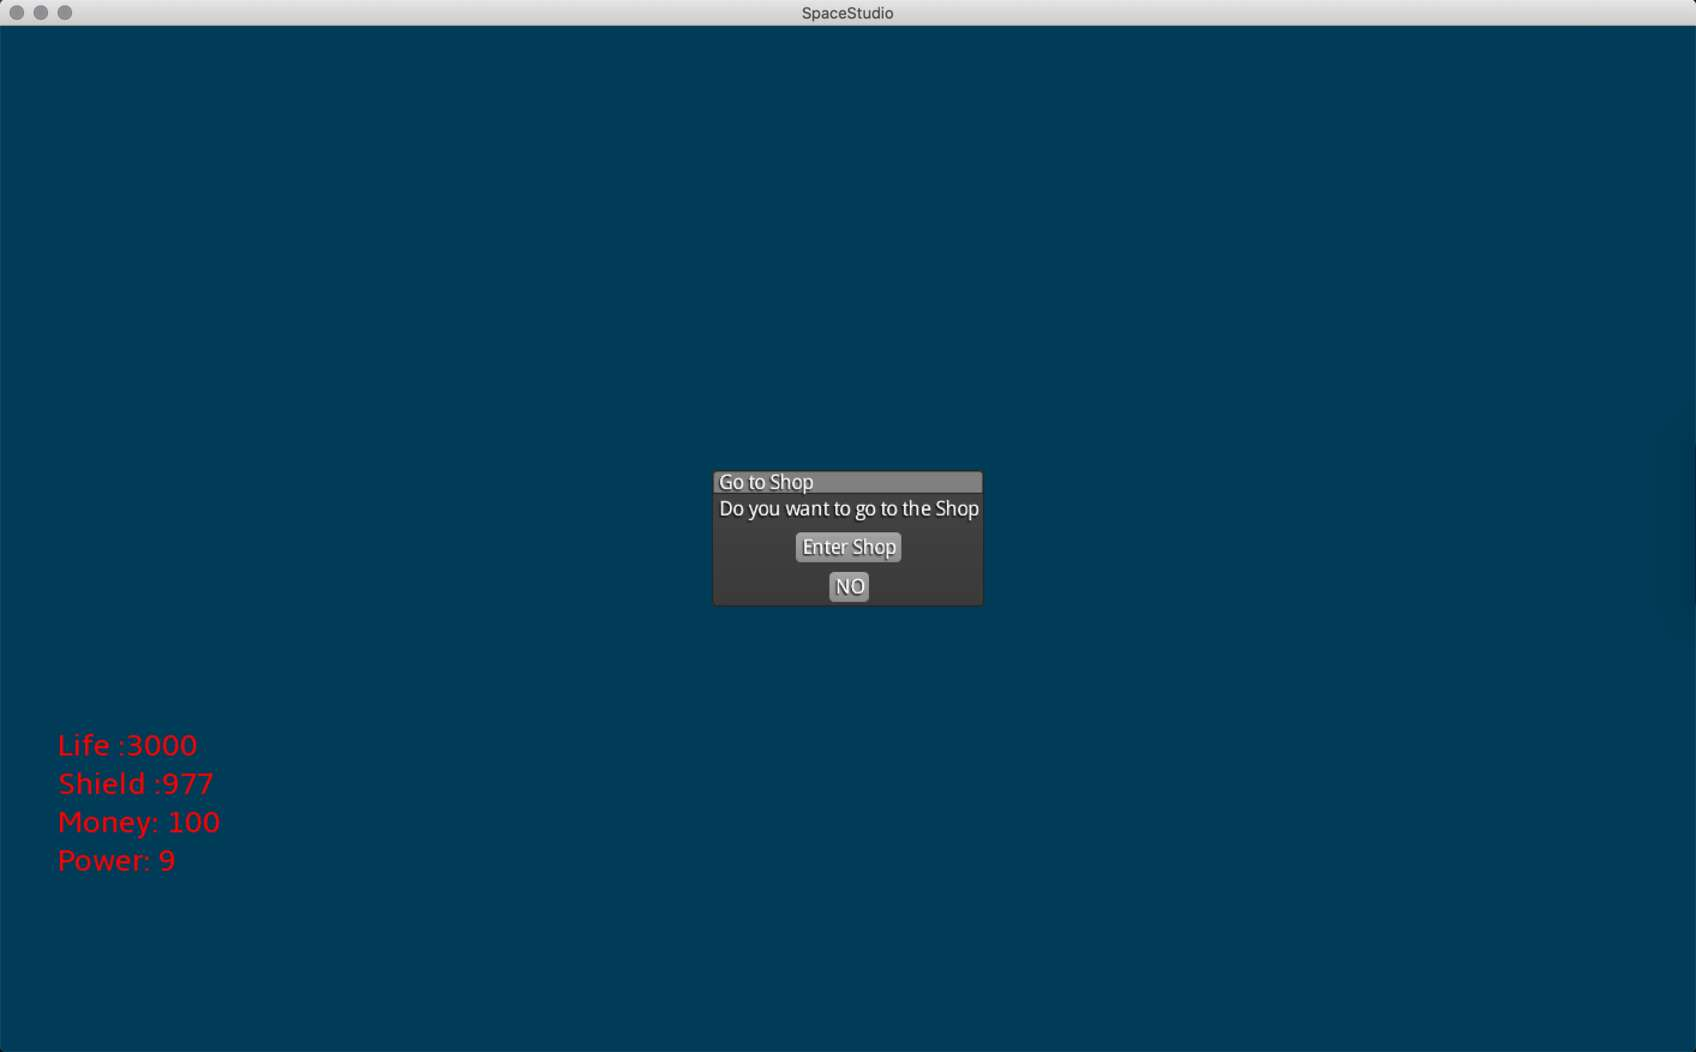
\includegraphics[scale=0.4]{TestProtocolBilder/shopPlanetJump.jpg}
\caption{Springen zur Shop-Station}
\end{figure}
\newpage
\section{Shop Screen}
Wenn der Benutzer den Shop-Bildschirm betritt, kann er den Kaufen-Button und die verfügbaren Ressourcen sehen.
\begin{figure}[h]
\centering
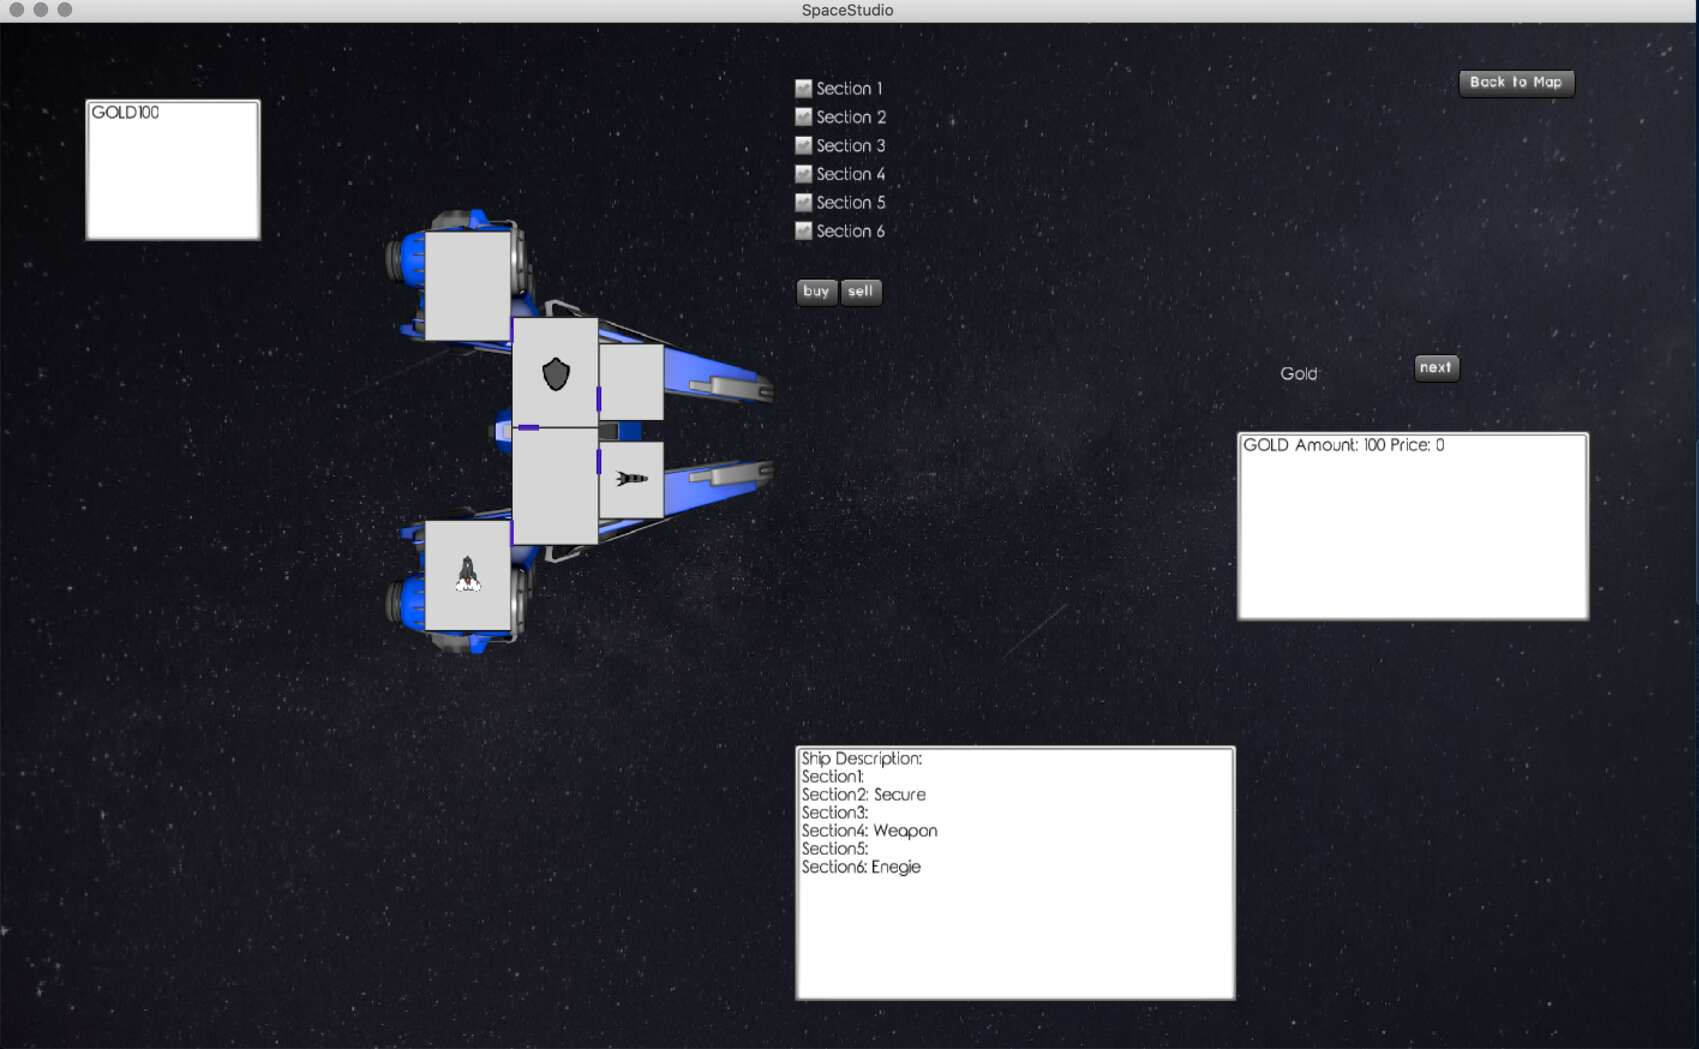
\includegraphics[scale=0.4]{TestProtocolBilder/shopScreen.jpg}
\caption{shop Screen}
\end{figure}

\subsection{kaufen}
Als nächstes wurde der Kauf jedes Objekts sowie das Ergebnis des verbleibenden Geldes des Spielers getestet.

\subsubsection{Gold kaufen}
Dies ist das Ergebnis nach dem Kauf von Gold, was sich direkt auf das Geld des Benutzers auswirkt.
\begin{figure}[htp]
\centering
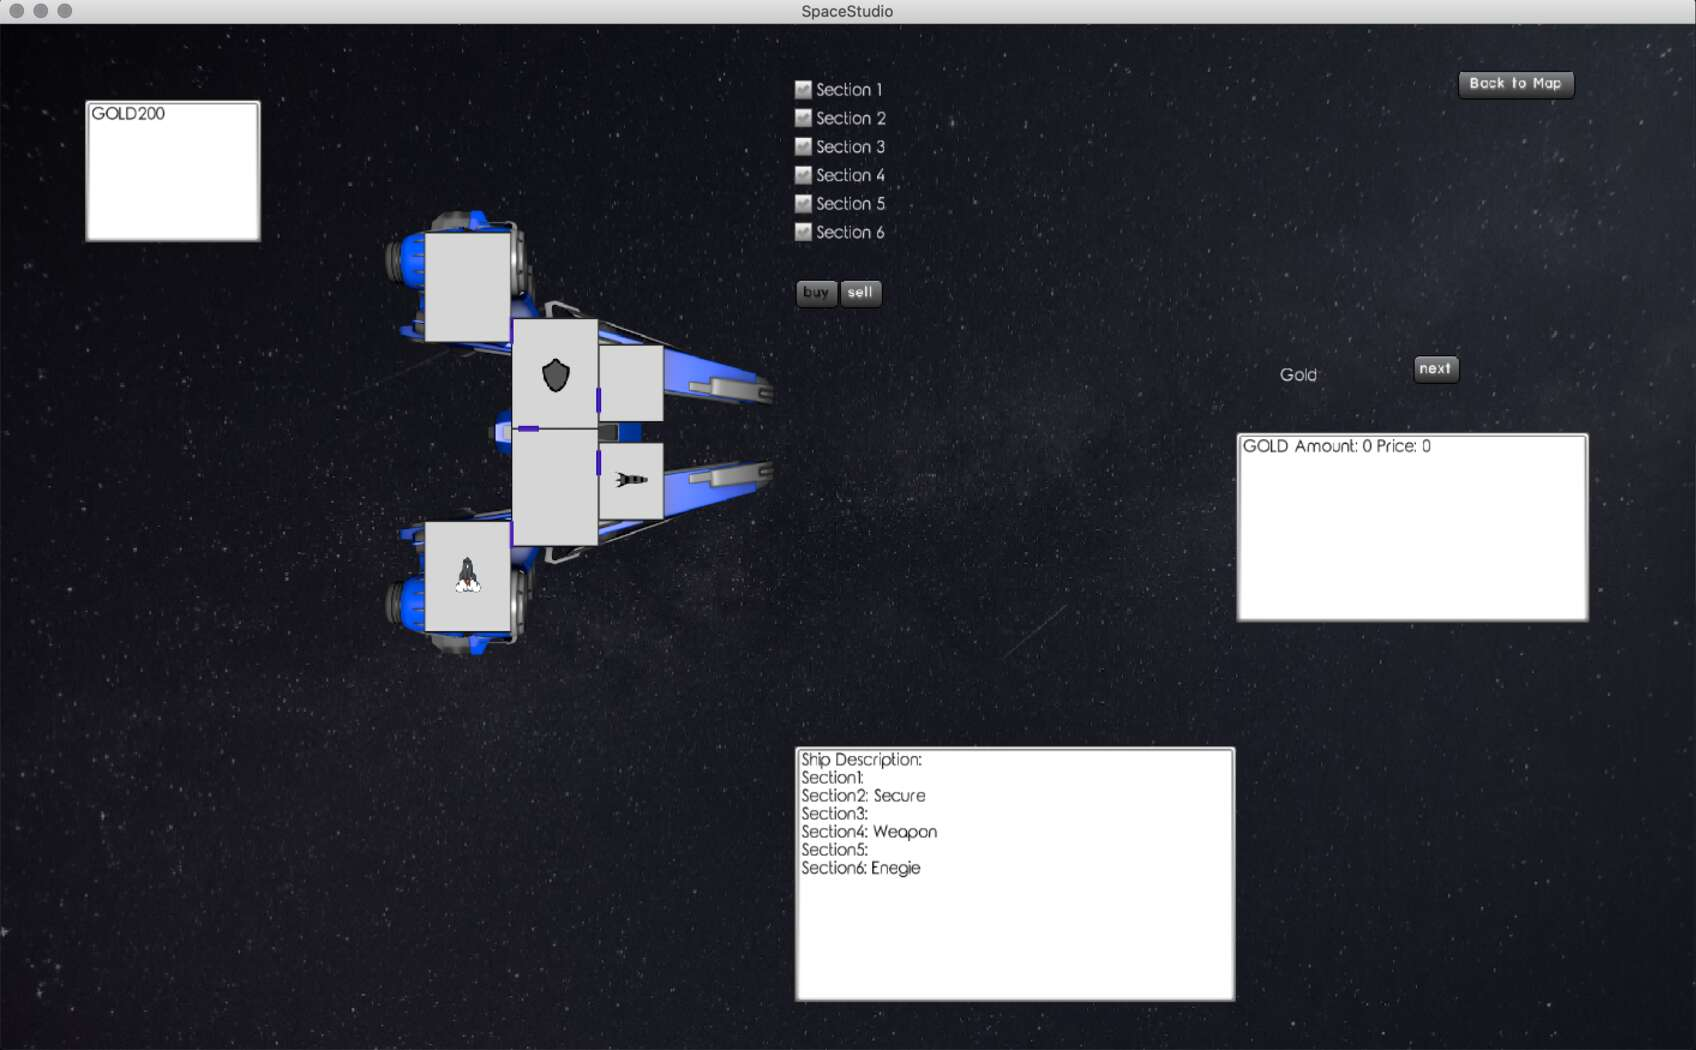
\includegraphics[scale=0.4]{TestProtocolBilder/goldgekauft.jpg}
\caption{Anderer Typ von Ereignissen}
\end{figure}
\newpage
\subsubsection{Energie kaufen}
Dies ist das Ergebnis nach dem Kauf von Energie. Dieser Kauf wirkt sich auf das Raumschiff aus und es ist nur möglich, die Reduzierung von Gold auf dem Boot zu sehen.
\begin{figure}[htp]
\centering
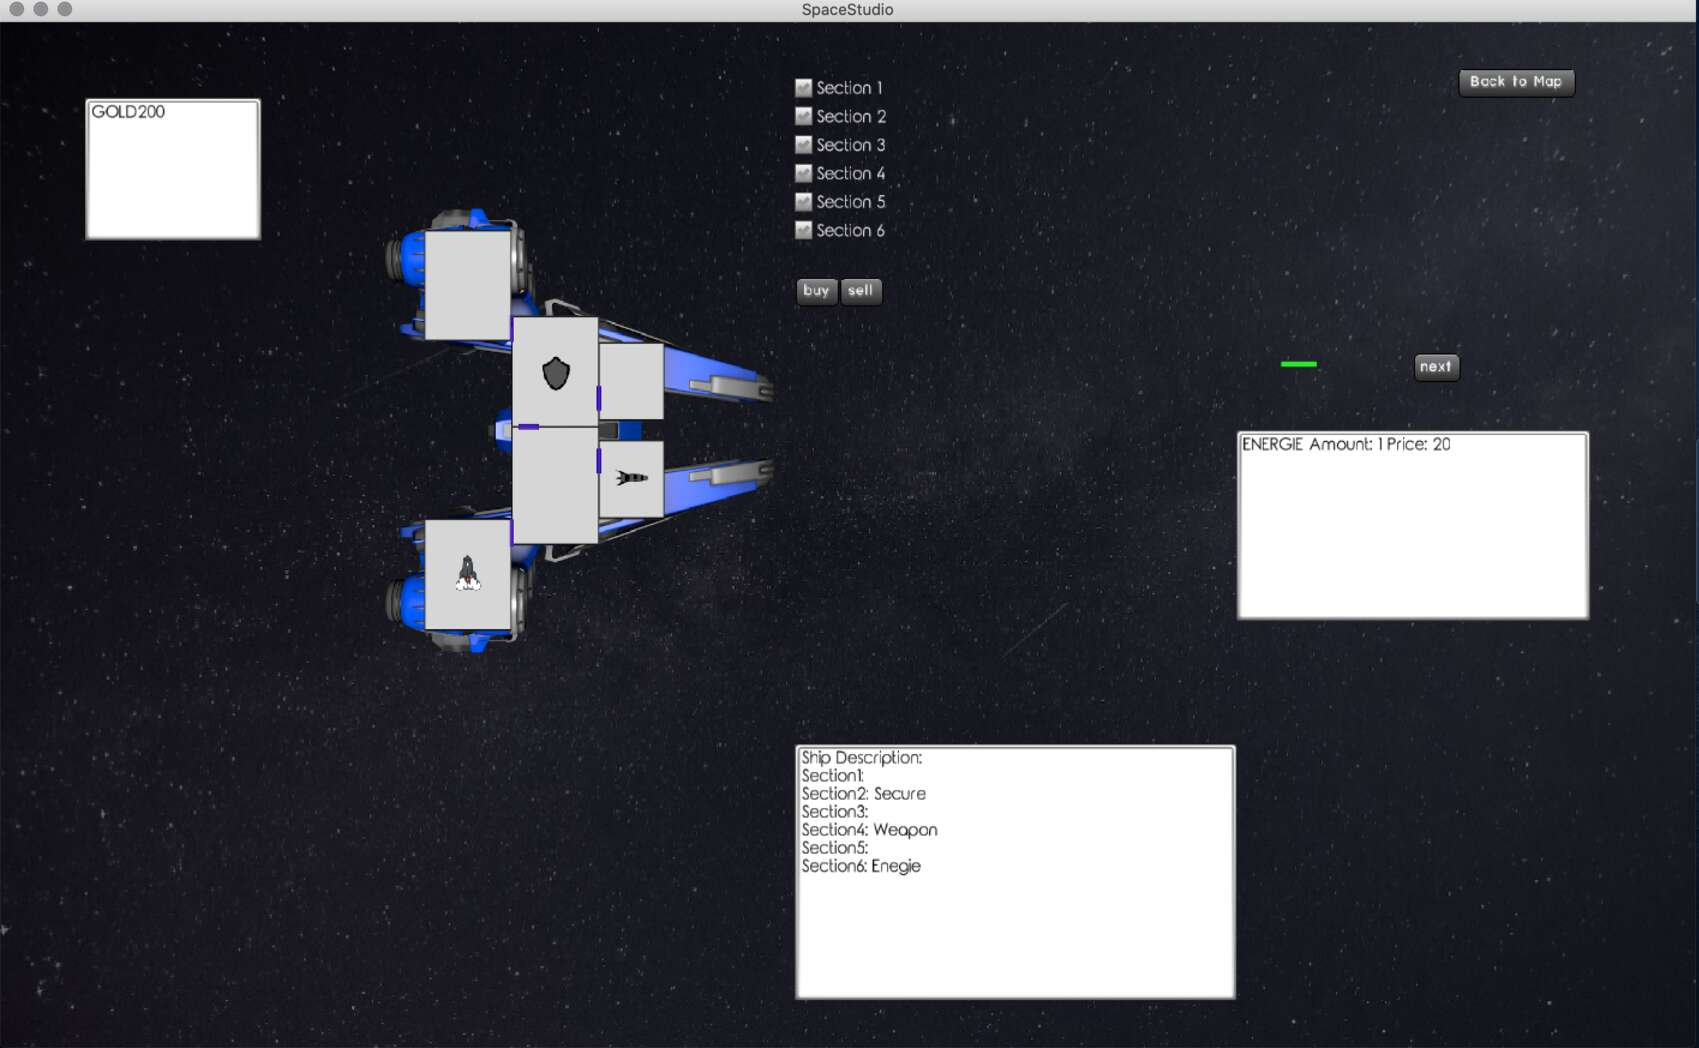
\includegraphics[scale=0.4]{TestProtocolBilder/energie.jpg}
\caption{andere Typ von Ereignisse}
\end{figure}
\newpage
\subsubsection{Waffen kaufen}
Der Kauf von Waffen wurde getestet, diese Aktion verringert das Gold des Spielers.    
\begin{figure}[htp]
\centering
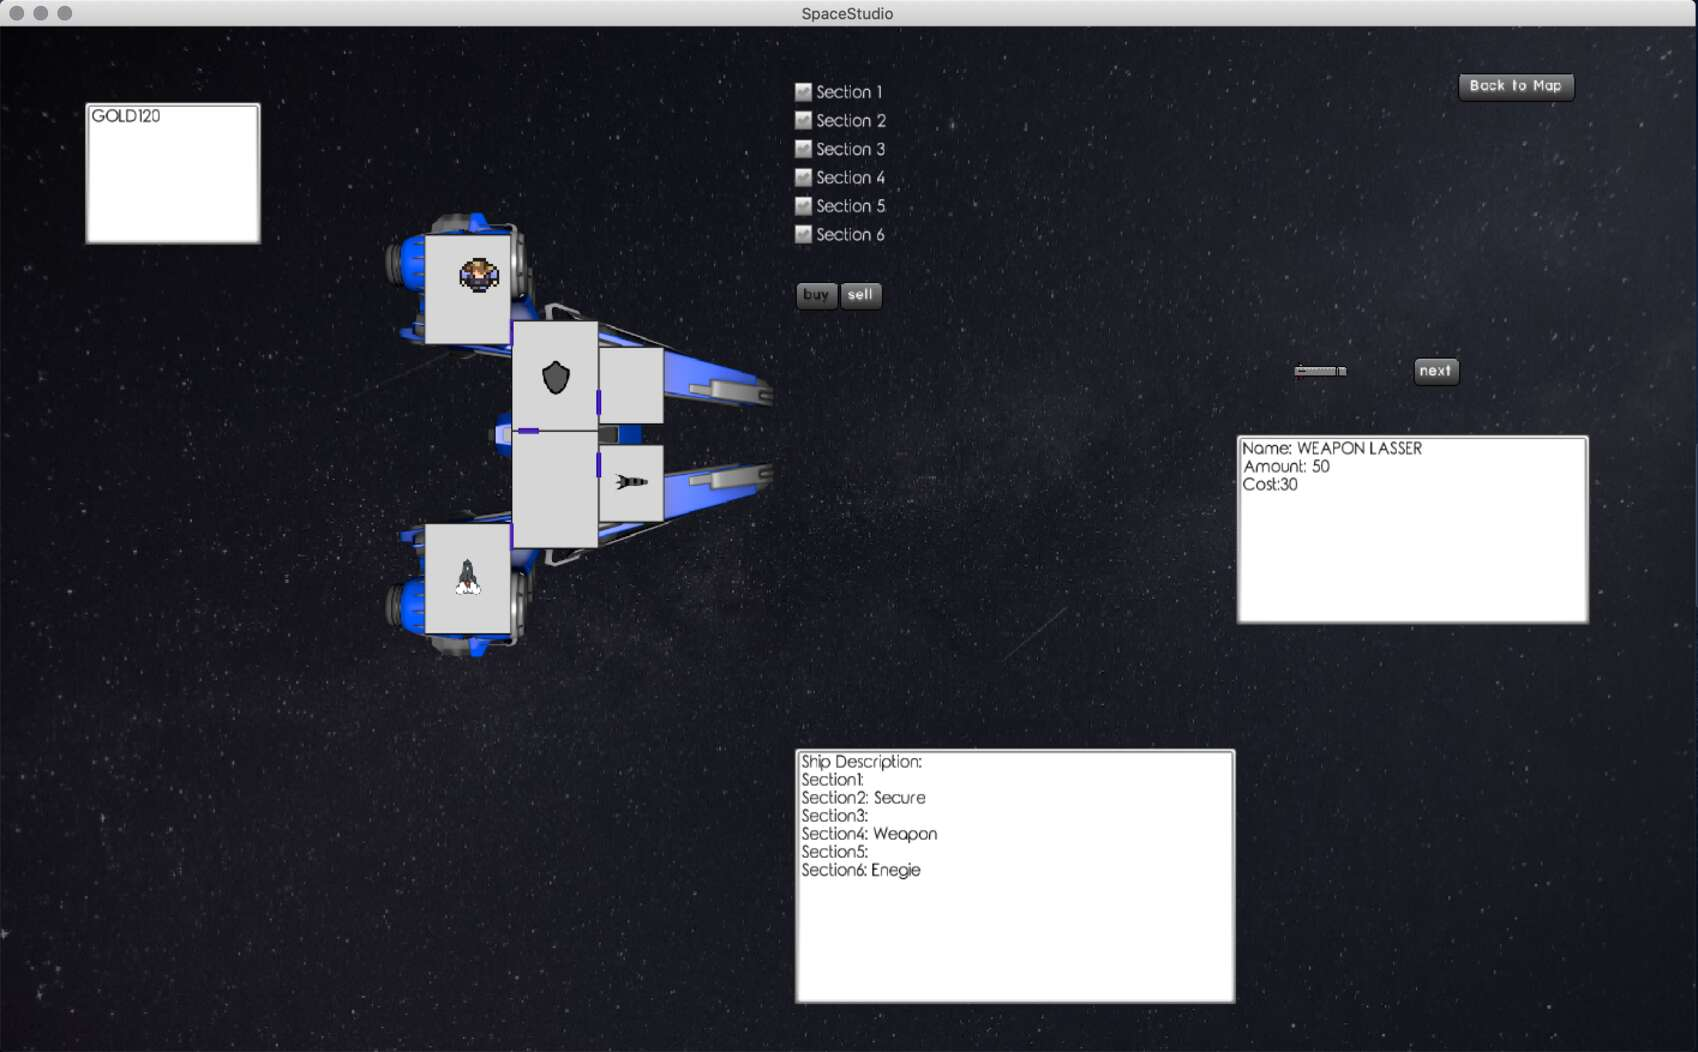
\includegraphics[scale=0.4]{TestProtocolBilder/weaponkaufen.jpg}
\caption{Anderer Typ von Ereignissen}
\end{figure}
\newpage
\subsubsection{Crewmember kaufen}
Beim Kauf von Mitgliedern wurde getestet, dass zuerst ein Abschnitt ausgewählt werden muss, in dem dieses Mitglied positioniert werden muss, wenn der Kauf getätigt werden kann.
\begin{figure}[htp]
\centering
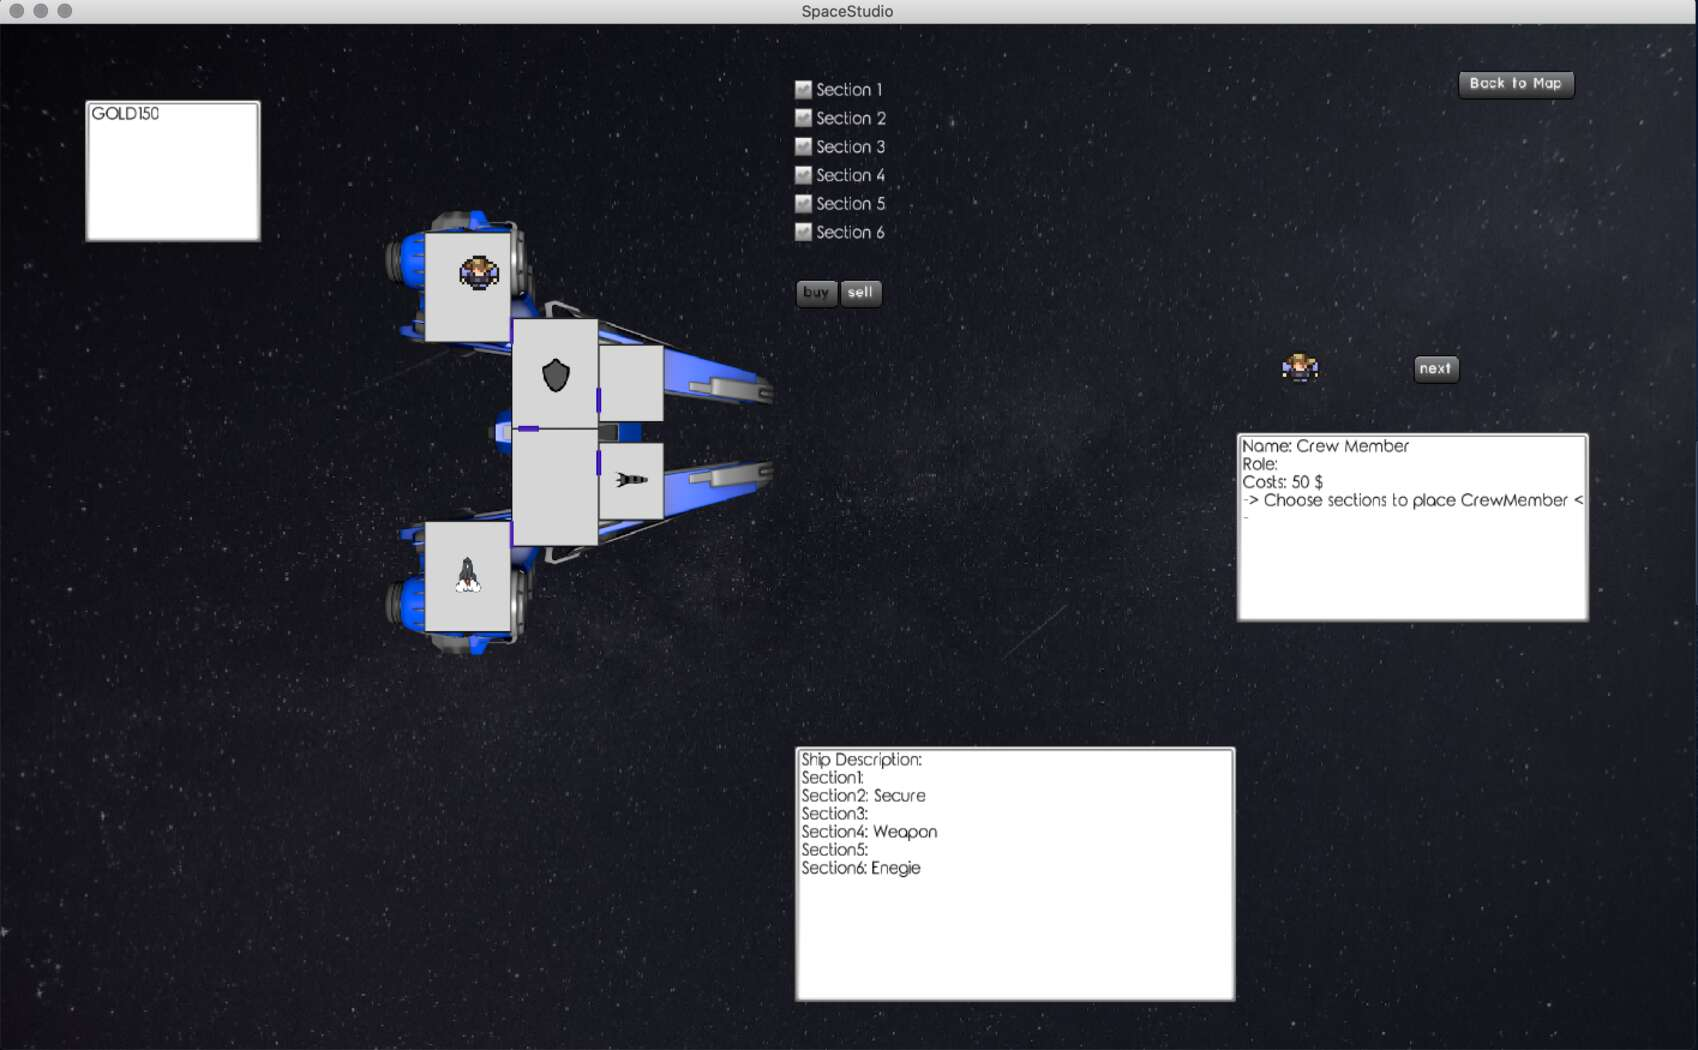
\includegraphics[scale=0.4]{TestProtocolBilder/crewmemberkaufen.jpg}
\caption{Anderer Typ von Ereignissen}
\end{figure}


\newpage
\section{Combat Screen}
Auf diesem Bildschirm wird jeder Knopf getestet und die Logik für einen Kampf ermittelt.

\subsection{Inital combat Screen}
Die Hauptschaltfläche auf dem Bildschirm ist der unterste Knopf, mit der Sie eine Runde starten oder beenden können. Dieser Button verringert das Aufwärmen und lässt Waffen schießen.
\begin{figure}[htp]
\centering
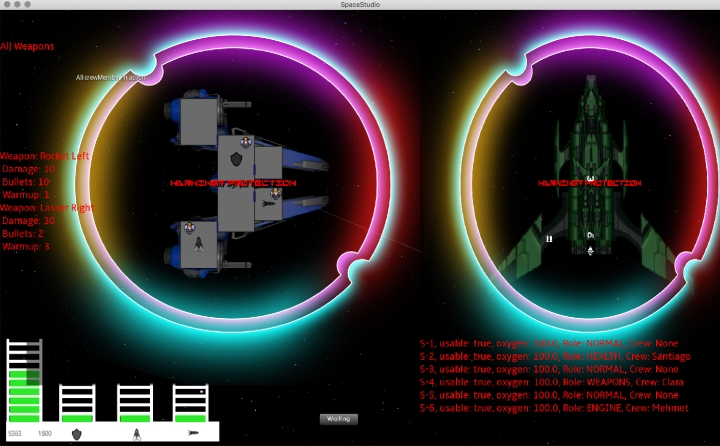
\includegraphics[scale=0.7]{TestProtocolBilder/OptimizedinitialBattelScreen.png}
\caption{Anderer Typ von Ereignissen}
\end{figure}

\newpage
\subsection{Energieverteilung}
Die Beschriftungen unten rechts ermöglichen es, den Zustand der Player zu kennen. Diese ändern sich dynamisch nach den Anweisungen des Spielers.
\begin{figure}[htp]
\centering
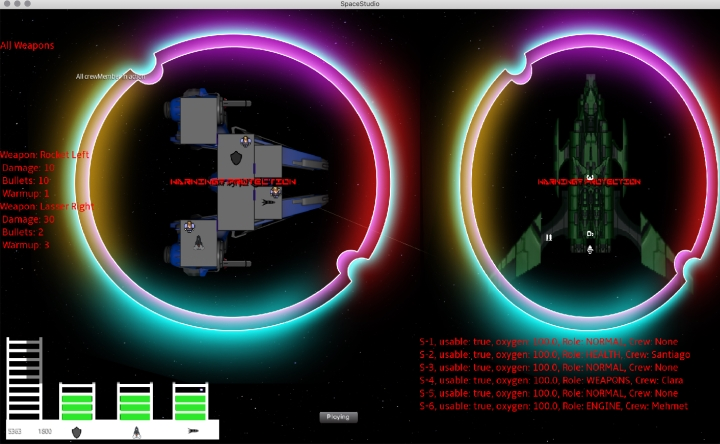
\includegraphics[scale=0.7]{TestProtocolBilder/OptimizedEnergieAlleSysteme.png}
\caption{Anderer Typ von Ereignissen}
\end{figure}

\newpage
\subsection{Keine Energie im Waffen System}
Jeder Knopf wurde getestet, um die Energie zu teilen, und es wurde getestet, dass das Waffensystem, wenn es keine Energie hat, nicht feuern kann.
\begin{figure}[htp]
\centering
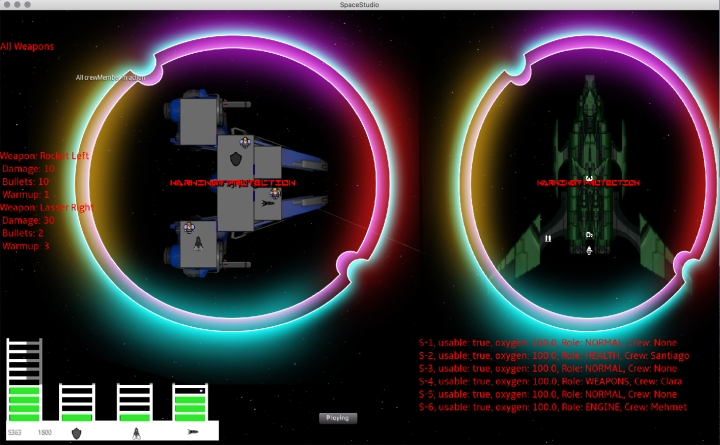
\includegraphics[scale=0.7]{TestProtocolBilder/OptimizedEnergieVerteilung.png}
\caption{Anderer Typ von Ereignissen}
\end{figure}

\newpage
\subsection{Gegner schießt}
Es wurde getestet, dass der Gegner, wenn er an der Reihe ist, schießen kann und die Kugeln in der grafischen Oberfläche gerendert werden.
\begin{figure}[htp]
\centering
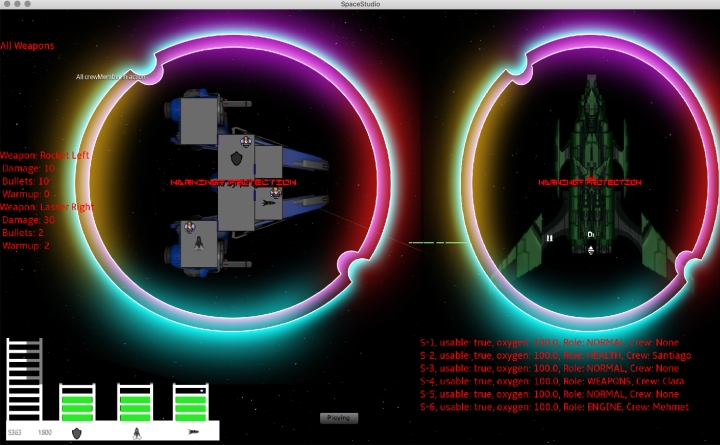
\includegraphics[scale=0.7]{TestProtocolBilder/OptimizedgegnerShots.png}
\caption{andere Typ von Ereignisse}
\end{figure}


\newpage
\subsection{Player schießt}
Es wurde auch getestet, dass der Benutzer feuern kann, sobald ein feindlicher Abschnitt ausgewählt wurde, dass das Aufwärmen Null ist und dass der Waffenabschnitt verwendbar ist. Auch, dass die Kugeln gerendert werden.
\begin{figure}[htp]
\centering
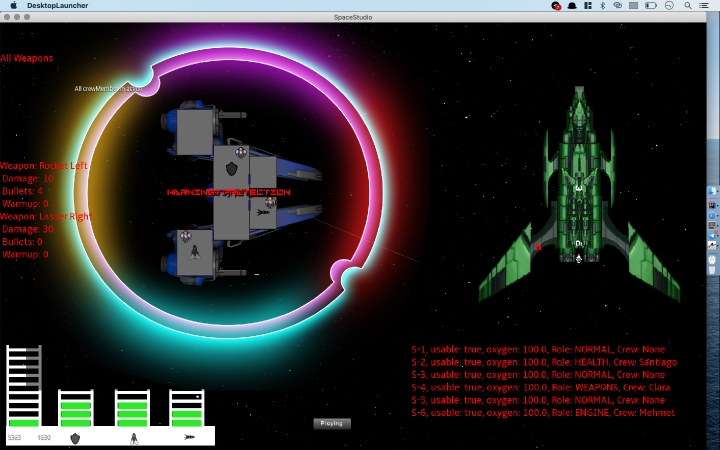
\includegraphics[scale=0.7]{TestProtocolBilder/OptimizedweaponsShot.png}
\caption{Waffen können wieder feuern, wenn das System eingeschaltet wurde.}
\end{figure}

\newpage
\subsection{Win Screen}
Es wurde getestet, dass der Benutzer beim Schießen des Spielers eine Verkürzung des Lebens des Gegners feststellen kann. Wenn dieses Leben Null erreicht, wird der Benutzer gewarnt, dass er weiterhin Planeten erforschen kann.
\begin{figure}[htp]
\centering
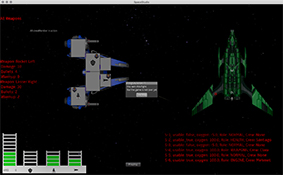
\includegraphics[scale=1.2]{TestProtocolBilder/wonScreen.jpg}
\caption{Win Screen, als der Feind besiegt wurde }
\end{figure}
\newpage
\subsection{Bewegung der Mitglieder}
Wenn ein Teammitglied aus dem Bereich verschoben wird, sehen Sie Symbole, wo dieses Teammitglied platziert werden kann.
\begin{figure}[htp]
\centering
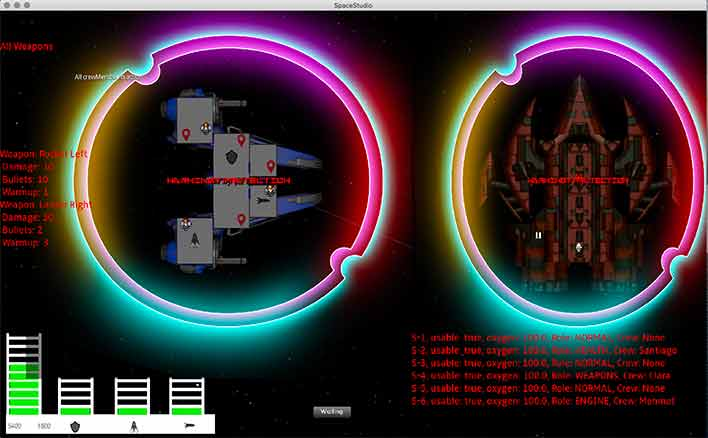
\includegraphics[scale=0.6]{TestProtocolBilder/crewmemberpull@0,25x.jpg}
\caption{Crewmember auf andere Sektionen bewegen}
\end{figure}
\newpage
\subsection{Wartezeit}
Es ist notwendig, einige Zeit zu warten, bis die Mitglieder, die geändert wurden, den Abschnitt erreichen. Deshalb ist das Sanduhrsymbol aufgesetzt. Diese Implementierung wurde erfolgreich getestet.
\begin{figure}[htp]
\centering
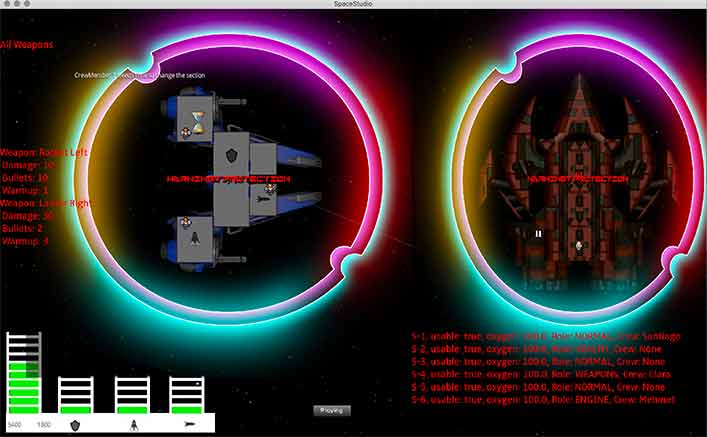
\includegraphics[scale=0.6]{TestProtocolBilder/timewaiting@0,25x.jpg}
\caption{Wartezeit für Crewmember Bewegungen}
\end{figure}
\newpage
\subsection{Dunkle Planeten}
Es wurde getestet, dass wenn der Benutzer vom Planeten springt, der besuchte Planet dunkel angezeigt wird, so dass der Benutzer weiß, welche Planeten er schon besucht hat.
\begin{figure}[htp]
\centering
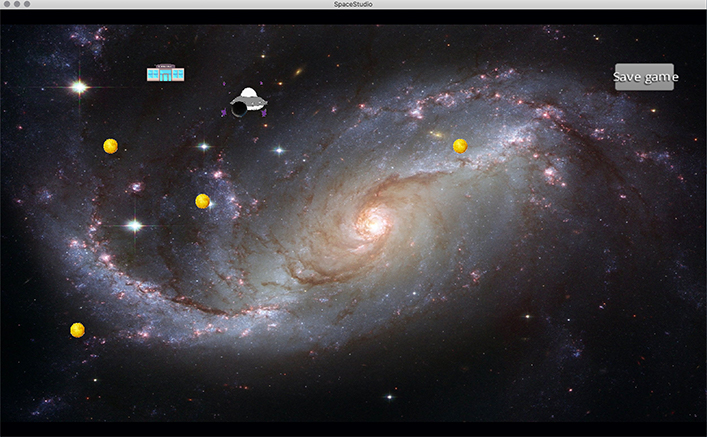
\includegraphics[scale=0.6]{TestProtocolBilder/besuchtePlanet.jpg}
\caption{Dunkle Planeten}
\end{figure}
\newpage
\subsection{Upgrade}
Wenn Sie auf die Schaltfläche Upgrade klicken, sehen Sie die möglichen Optionen zur Verbesserung des Schiffs des Spielers.
\begin{figure}[htp]
\centering
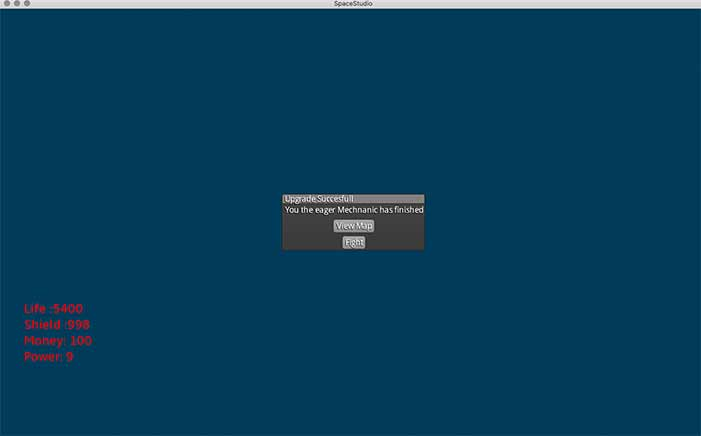
\includegraphics[scale=0.6]{TestProtocolBilder/nachupgrade@0,25x.jpg}
\caption{Upgrade Optionen}
\end{figure}

Wenn ein Upgrade ausgewählt wurde, können Sie mit dem Kampfbildschirm fortfahren.
\begin{figure}[htp]
\centering
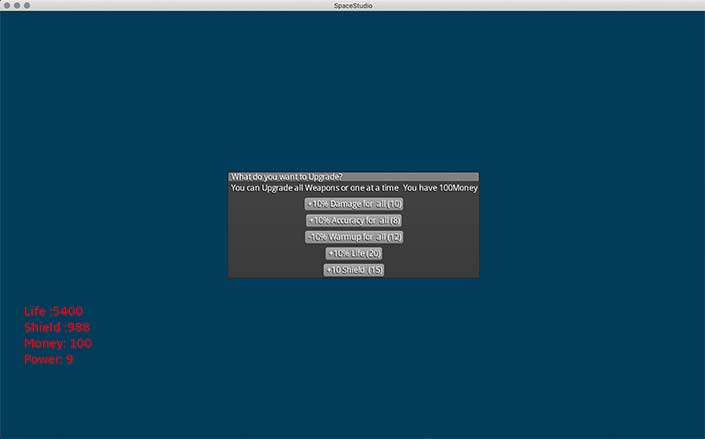
\includegraphics[scale=0.6]{TestProtocolBilder/upgrade@0,25x.jpg}
\caption{Nach Upgrade zum Combat Screen}
\end{figure}
\end{document}

